\chapter{序列二次规划}
\label{chap:sequential-quadratic-programming}

考虑圆周上的一个小问题：
\begin{equation}
 \min_{\bm{x}\in\mathbb{R}^2}\ f(\bm{x})=-x_1-x_2
 \quad\text{s.t.}\quad h(\bm{x})=x_1^2+x_2^2-2=0.
 \label{eq:sqp-circle}
\end{equation}
解是$\bm{x}^\star=(1,1)^\top$。第~\ref{chap:penalty-multiplier-methods}章的办法是把约束折进目标，解一串无约束问题，每个无约束问题自身又要迭代很多步。第~\ref{chap:second-order-methods}章的Newton法提示了另一条路：在当前点建一个局部模型，一步解出模型的最优步，再换一个点重建模型。

把这个想法搬到约束问题上，立刻有几个问题。约束也要进入模型，它该近似到几阶？式~\eqref{eq:sqp-circle}的目标是线性的，Hessian为零，模型的曲率从哪里来？约束不止一条时，哪些不等式此刻该算数？模型给出的步不满足真实约束，也未必降低目标，又凭什么采用它？

本章按这个顺序回答。第~\ref{sec:sqp-local-model}节写出局部模型，它是一个二次规划。第~\ref{sec:sqp-equality-qp}节解只含等式的模型，第~\ref{sec:sqp-active-set}节处理不等式。第~\ref{sec:sqp-curvature}节讨论模型的曲率不合适时怎么办。

第~\ref{sec:sqp-acceptance}节把模型的步放回原问题检验，第~\ref{sec:sqp-repair}节处理模型本身失效或好步被误拒的情形。第~\ref{sec:sqp-convergence}节说明这些部件合起来在什么条件下收敛得快，以及每一轮要花多少计算。全章用问题~\eqref{eq:sqp-circle}作手算的主线。

\section{局部二次模型}
\label{sec:sqp-local-model}

站在当前点$\bm{x}^{(t)}$，怎样写出一个既能求解、又能代表原问题的局部模型？一般的问题写成
\begin{equation}
 \begin{aligned}
 \min_{\bm{x}\in\mathbb{R}^n}\quad & f(\bm{x})\\
 \text{s.t.}\quad & g_i(\bm{x})\leq0,\quad i=1,\ldots,m,\\
 & h_j(\bm{x})=0,\quad j=1,\ldots,p,
 \end{aligned}
 \label{eq:sqp-nlp}
\end{equation}
其中$f,g_i,h_j$都二阶连续可微。

\paragraph{约束怎样近似}
Newton法把目标近似到二阶。约束若也近似到二阶，模型的可行域由二次曲面围成，这样的子问题本身就难解。所以约束只取一阶，用切平面代替曲面。记$\bm{d}$为待求的步，把约束的值和梯度在$\bm{x}^{(t)}$处取定，有
\[
 h_j(\bm{x}^{(t)}+\bm{d})\approx h_j(\bm{x}^{(t)})+\langle\nabla h_j(\bm{x}^{(t)}),\bm{d}\rangle.
\]

把各条约束的梯度按行排成Jacobian矩阵，记$\bm{A}^{(t)}\in\mathbb{R}^{p\times n}$的第$j$行为$\nabla h_j(\bm{x}^{(t)})^\top$，$\bm{G}^{(t)}\in\mathbb{R}^{m\times n}$的第$i$行为$\nabla g_i(\bm{x}^{(t)})^\top$。约束的值记作向量$\bm{h}^{(t)}$和$\bm{g}^{(t)}$。这样，要求线性化后的约束成立就是
\begin{equation}
 \bm{h}^{(t)}+\bm{A}^{(t)}\bm{d}=\bm{0},\qquad \bm{g}^{(t)}+\bm{G}^{(t)}\bm{d}\leq\bm{0}.
 \label{eq:sqp-linearized}
\end{equation}

以问题~\eqref{eq:sqp-circle}为例，从$\bm{x}^{(0)}=(1.5,0.5)^\top$出发。约束的值和梯度是
\[
 h^{(0)}=2.25+0.25-2=0.5,\qquad \bm{A}^{(0)}=(3,1).
\]

线性化约束于是成为
\[
 3d_1+d_2+0.5=0.
\]
图~\ref{fig:sqp-circle-model}(a)中的虚线就是这条直线。$\bm{x}^{(0)}$在圆外，过它有一条等值线$h=0.5$。虚线与这条等值线在$\bm{x}^{(0)}$处的切线平行，并向圆的方向平移，平移量按一阶估计恰好抵消$h^{(0)}=0.5$的违约。

\begin{BookInlineFigure}
 \centering
 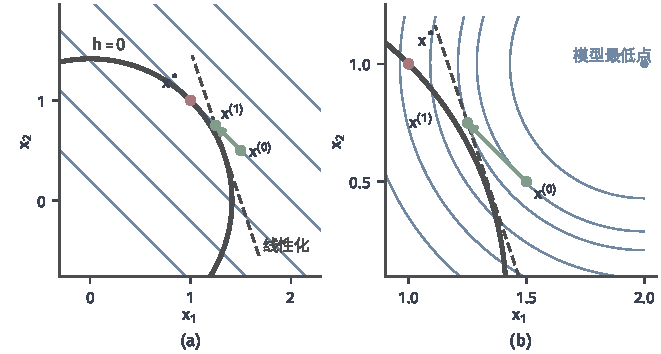
\includegraphics[width=112mm]{figures/05-optimization/06-constrained-optimization/matplotlib/sqp-circle-model/figure.pdf}
 \caption{问题~\eqref{eq:sqp-circle}的第一个局部模型。深灰粗线是圆$h=0$，虚线是线性化约束，绿点是迭代点，红点是解。(a)~蓝色直线是目标的等值线，步落在虚线上而不在圆上。(b)~放大的局部，蓝色圆是取$\bm{B}^{(0)}=2\bm{I}$时模型的等值线，模型无约束的最低点在右上方，受虚线限制后，最优步停在等值线与虚线相切的地方。}
 \label{fig:sqp-circle-model}
\end{BookInlineFigure}

\paragraph{目标怎样近似}
目标的一阶项仍取$\langle\nabla f(\bm{x}^{(t)}),\bm{d}\rangle$，二次项用一个对称矩阵$\bm{B}^{(t)}$。把两部分合起来，就得到局部模型。下面的定义里$\bm{B}^{(t)}$暂时留作待定，它的选取马上讨论。

\begin{definition}[局部二次规划与SQP]
\label{def:sqp-subproblem}
给定当前点$\bm{x}^{(t)}$与对称矩阵$\bm{B}^{(t)}$，\term{局部二次规划}（local quadratic program）是以$\bm{d}\in\mathbb{R}^n$为未知量的问题
\begin{equation}
 \begin{aligned}
 \min_{\bm{d}}\quad & \langle\nabla f(\bm{x}^{(t)}),\bm{d}\rangle+\frac12\bm{d}^\top\bm{B}^{(t)}\bm{d}\\
 \text{s.t.}\quad & \bm{h}^{(t)}+\bm{A}^{(t)}\bm{d}=\bm{0},\\
 & \bm{g}^{(t)}+\bm{G}^{(t)}\bm{d}\leq\bm{0}.
 \end{aligned}
 \label{eq:sqp-qp}
\end{equation}
反复构造并求解这样的子问题、用其解更新迭代点和乘子的方法，称为\term{序列二次规划}（sequential quadratic programming，SQP）。
\end{definition}

目标是二次的、约束是线性的，这就是第~\ref{chap:quadratic-conic-programming}章的二次规划（QP）。每一项的职责不同：目标梯度指出一阶意义下该往哪里走；$\bm{h}^{(t)},\bm{g}^{(t)}$说明当前违约多少；两个Jacobian说明约束怎样随步变化；$\bm{B}^{(t)}$说明走远了之后模型该怎样弯曲。

\paragraph{曲率为什么不能只取目标的Hessian}
最自然的想法是令$\bm{B}^{(t)}=\nabla^2f(\bm{x}^{(t)})$。式~\eqref{eq:sqp-circle}直接否定了这个想法。这里$\nabla^2f=\bm{0}$，模型的目标退化成线性函数，而可行集是一条直线，只要目标沿这条直线的斜率不为零，模型就没有下界。可是真实问题在圆上明明有一个弯曲的碗。

这只碗来自约束的弯曲。设想沿圆周走：坐标$x_1,x_2$本身在转弯，所以线性函数$f$沿圆周读出来的数值是弯的。模型把圆拉直成了直线，这部分弯曲必须另外算回目标的二次项。

下面把这件事算清楚。设$\bm{x}(s)$是一条留在等式约束上的光滑曲线，它在$s=0$处经过$\bm{x}$，速度是$\bm{v}$，加速度是$\bm{w}$。对恒等式$h_j(\bm{x}(s))=0$在$s=0$处求两次导数，得到
\[
 \langle\nabla h_j(\bm{x}),\bm{v}\rangle=0,\qquad
 \langle\nabla h_j(\bm{x}),\bm{w}\rangle+\bm{v}^\top\nabla^2h_j(\bm{x})\bm{v}=0.
\]

目标沿这条曲线的二阶导数由链式法则给出，它含有加速度$\bm{w}$：
\[
 \frac{\mathrm{d}^2}{\mathrm{d}s^2}f(\bm{x}(s))\Big|_{s=0}
 =\bm{v}^\top\nabla^2f(\bm{x})\bm{v}+\langle\nabla f(\bm{x}),\bm{w}\rangle.
\]

第~\ref{chap:constrained-optimality}章的一阶条件说，KKT点上$\nabla f+\sum_j\nu_j\nabla h_j=\bm{0}$，这里记Lagrange函数为$\mathcal{L}=f+\sum_i\lambda_ig_i+\sum_j\nu_jh_j$。把$\nabla f$代换掉，再用前面关于$\bm{w}$的恒等式，得到
\[
 \langle\nabla f,\bm{w}\rangle=-\sum_j\nu_j\langle\nabla h_j,\bm{w}\rangle=\sum_j\nu_j\bm{v}^\top\nabla^2h_j\bm{v}.
\]

代回上式，加速度消失了，剩下的正是Lagrange函数的Hessian：
\begin{equation}
 \frac{\mathrm{d}^2}{\mathrm{d}s^2}f(\bm{x}(s))\Big|_{s=0}
 =\bm{v}^\top\nabla^2_{\bm{x}\bm{x}}\mathcal{L}(\bm{x},\bm{\nu})\bm{v}.
 \label{eq:sqp-curve-curvature}
\end{equation}
这里乘子把约束的弯曲折算成了目标的弯曲，它正是第~\ref{chap:constrained-optimality}章二阶条件里出现$\nabla^2_{\bm{x}\bm{x}}\mathcal{L}$的原因。活动的不等式在其边界上同样处理，不活动的不等式乘子为零，不贡献曲率。

在圆上验证一下。沿圆取弧长参数$s$，解$\bm{x}^\star$处的乘子由$(-1,-1)^\top+\nu(2,2)^\top=\bm{0}$得$\nu^\star=1/2$，于是
\[
 \nabla^2_{\bm{x}\bm{x}}\mathcal{L}=2\nu^\star\bm{I}=\bm{I}.
\]

单位切向量$\bm{v}$给出$\bm{v}^\top\bm{I}\bm{v}=1$。另一方面，沿圆有$f=-2\cos(s/\sqrt2)$，它在$s=0$处的二阶导数是
\[
 \frac{\mathrm{d}^2f}{\mathrm{d}s^2}\Big|_{s=0}=2\cdot\frac12=1,
\]
两者相等。图~\ref{fig:sqp-curvature-circle}(a)画的就是这件事：带Lagrange曲率的模型与圆上的目标贴合，只用$\nabla^2f$的模型是一条平线。

\begin{BookInlineFigure}
 \centering
 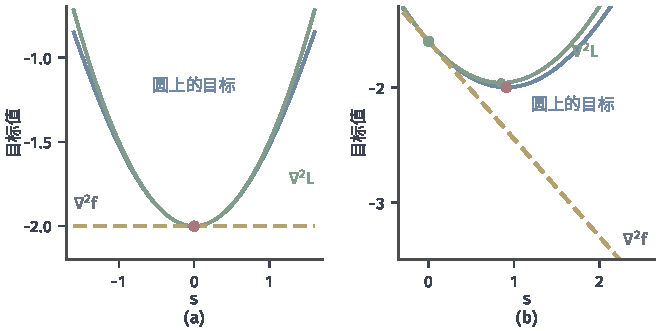
\includegraphics[width=112mm]{figures/05-optimization/06-constrained-optimization/matplotlib/sqp-curvature-along-circle/figure.pdf}
 \caption{沿约束的目标与两种模型，$s$是弧长（对模型是沿切线的距离）。蓝线是圆上真实的目标；绿线的二次项取$\nabla^2_{\bm{x}\bm{x}}\mathcal{L}=\bm{I}$；黄色虚线的二次项取$\nabla^2f=\bm{0}$。(a)~在解$\bm{x}^\star$处（红点）。(b)~在圆上的点$(1.4,0.2)^\top$处（左侧绿点）：绿色模型的最低点靠近真实最低点，只用$\nabla^2f$的模型沿切线一路下降，没有下界。}
 \label{fig:sqp-curvature-circle}
\end{BookInlineFigure}

式~\eqref{eq:sqp-curve-curvature}的推导用到了KKT点上的梯度关系，所以严格说它是解处的性质。迭代中手里只有估计值，于是取
\begin{equation}
 \bm{B}^{(t)}=\nabla^2_{\bm{x}\bm{x}}\mathcal{L}(\bm{x}^{(t)},\bm{\lambda}^{(t)},\bm{\nu}^{(t)})
 =\nabla^2f+\sum_{i=1}^m\lambda_i^{(t)}\nabla^2g_i+\sum_{j=1}^p\nu_j^{(t)}\nabla^2h_j,
 \label{eq:sqp-lagrangian-hessian}
\end{equation}
右端都在$\bm{x}^{(t)}$处取值，或取它的近似（第~\ref{sec:sqp-quasi-newton}节）。这解释了SQP为什么要同时维护原始变量和乘子：没有乘子，就写不出模型的曲率。

图~\ref{fig:sqp-curvature-circle}(b)显示了乘子估计不太准时的情形。点$(1.4,0.2)^\top$在圆上但不是解，取$\nu=1/2$，绿色模型的最低点仍然靠近真实的最低点。类比“局部模型信多远”：线性化约束告诉我们该待在哪里，乘子曲率告诉我们沿着允许的方向能走多远。这个类比在远离解时失效，那时乘子可能是错的，模型未必是碗，这是第~\ref{sec:sqp-curvature}节的话题。

\paragraph{子问题的乘子}
QP也有自己的乘子。记不等式的乘子为$\hat{\bm{\lambda}}$，等式的乘子为$\hat{\bm{\nu}}$。线性约束本身满足约束资格，所以把第~\ref{chap:constrained-optimality}章的KKT条件用于式~\eqref{eq:sqp-qp}时，它的每个局部解都满足
\begin{equation}
 \begin{gathered}
 \bm{B}^{(t)}\bm{d}+\nabla f(\bm{x}^{(t)})+(\bm{A}^{(t)})^\top\hat{\bm{\nu}}+(\bm{G}^{(t)})^\top\hat{\bm{\lambda}}=\bm{0},\\
 \bm{h}^{(t)}+\bm{A}^{(t)}\bm{d}=\bm{0},\qquad \bm{g}^{(t)}+\bm{G}^{(t)}\bm{d}\leq\bm{0},\\
 \hat{\bm{\lambda}}\geq\bm{0},\qquad \hat\lambda_i\bigl(g_i^{(t)}+\langle\nabla g_i^{(t)},\bm{d}\rangle\bigr)=0,\quad i=1,\ldots,m.
 \end{gathered}
 \label{eq:sqp-qp-kkt}
\end{equation}

把$\bm{d}=\bm{0}$代入式~\eqref{eq:sqp-qp-kkt}，第一行成为原问题的Lagrange驻定条件，第二行成为原问题的可行性，第三行成为原问题的乘子非负与互补。这就是下面的引理，它说明模型和原问题在解处是一致的。

\begin{lemma}[零步与KKT点]
\label{lem:sqp-zero-step}
$\bm{d}=\bm{0}$连同乘子$(\hat{\bm{\lambda}},\hat{\bm{\nu}})$满足式~\eqref{eq:sqp-qp-kkt}，当且仅当$(\bm{x}^{(t)},\hat{\bm{\lambda}},\hat{\bm{\nu}})$满足原问题~\eqref{eq:sqp-nlp}的KKT条件。
\end{lemma}

\begin{proof}
令$\bm{d}=\bm{0}$，含$\bm{B}^{(t)}$的项消失，线性化项都等于在$\bm{x}^{(t)}$处的取值。式~\eqref{eq:sqp-qp-kkt}逐行就是原问题在$\bm{x}^{(t)}$处的驻定、可行、乘子非负和互补条件，反过来也一样。
\end{proof}

引理与$\bm{B}^{(t)}$无关，所以不论曲率怎样近似，模型的不动点都是原问题的KKT点。曲率只影响走向这个点的速度。解完QP后，新的乘子估计可以直接取子问题的乘子，当步长$\alpha^{(t)}\in(0,1]$时按比例插值：
\begin{equation}
 \begin{aligned}
 \bm{\lambda}^{(t+1)}&=\bm{\lambda}^{(t)}+\alpha^{(t)}\bigl(\hat{\bm{\lambda}}-\bm{\lambda}^{(t)}\bigr),\\
 \bm{\nu}^{(t+1)}&=\bm{\nu}^{(t)}+\alpha^{(t)}\bigl(\hat{\bm{\nu}}-\bm{\nu}^{(t)}\bigr).
 \end{aligned}
 \label{eq:sqp-multiplier-update}
\end{equation}

\paragraph{一轮计算的结构}
图~\ref{fig:sqp-loop}把一轮计算的部件排在一起。求值之后得到子问题，子问题给出步和乘子，步还要放回原问题检验。两处可能出岔：子问题可能无解，步也可能被拒绝。后面各节依次处理这些部件。

\begin{BookInlineFigure}
 \centering
 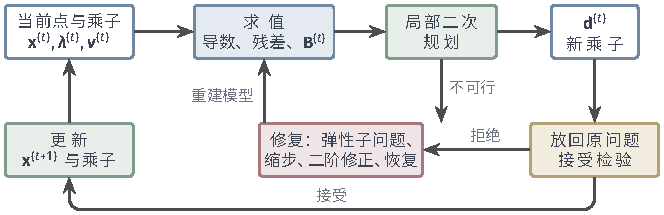
\includegraphics[width=112mm]{figures/05-optimization/06-constrained-optimization/tikz/sqp-loop/figure.pdf}
 \caption{SQP一轮计算的结构。绿框是模型的构造与接受后的更新，黄框是把步放回非线性问题的检验，红框是子问题无解或候选步被拒绝时的修复。修复之后重新建模或重新求解。}
 \label{fig:sqp-loop}
\end{BookInlineFigure}

需要说明的是，SQP规定的是“解一列局部QP”，并没有规定用什么方法解QP。下面用有效集法讲解，因为它的逻辑最贴近“哪些约束算数”这个问题；QP也可以用内点法或其他方法求解，第~\ref{chap:nonlinear-interior-point}章的内点法思想同样适用于QP。

局部模型还有一点要记住：模型可行不等于原问题可行。式~\eqref{eq:sqp-linearized}只是切平面，步$\bm{d}$落在切平面上，一般不在原来的曲面上。这个缺口贯穿全章，第~\ref{sec:sqp-acceptance}节和第~\ref{sec:sqp-repair}节专门处理它。

\section{等式QP的求解}
\label{sec:sqp-equality-qp}

式~\eqref{eq:sqp-qp}只含等式时，怎样求出它的解，这个解又在什么条件下才算数？这是SQP最基本的一步，下一节处理不等式时，每一轮要解的也是这种问题。为减少上标，本节在不引起混淆时省去$(t)$，并记$\bm{g}=\nabla f(\bm{x}^{(t)})$。

\paragraph{KKT线性系统}
只含等式时，条件~\eqref{eq:sqp-qp-kkt}的第一、二行就是全部要求。它们对$(\bm{d},\hat{\bm{\nu}})$是线性的，合起来写成块方程
\begin{equation}
 \underbrace{\begin{bmatrix}\bm{B}&\bm{A}^\top\\\bm{A}&\bm{0}\end{bmatrix}}_{\bm{K}}
 \begin{bmatrix}\bm{d}\\\hat{\bm{\nu}}\end{bmatrix}
 =-\begin{bmatrix}\bm{g}\\\bm{h}\end{bmatrix}.
 \label{eq:sqp-kkt-system}
\end{equation}
矩阵$\bm{K}\in\mathbb{R}^{(n+p)\times(n+p)}$称为\term{KKT矩阵}（KKT matrix）。它对称但不定，零对角块使它不可能正定，所以不能用Cholesky分解。

这个方程有解并不等于模型有最小点。要回答后一个问题，得看$\bm{B}$在允许的方向上是否向上弯。允许的方向是满足$\bm{A}\bm{v}=\bm{0}$的方向，它们构成$\bm{A}$的零空间。取矩阵$\bm{Z}\in\mathbb{R}^{n\times(n-p)}$，其各列构成这个零空间的一组基，就把问题缩到这$n-p$维上。矩阵$\bm{Z}^\top\bm{B}\bm{Z}$称为\term{约化Hessian}（reduced Hessian）。

\begin{theorem}[等式QP的可解性]
\label{thm:sqp-eqp}
设$\bm{A}\in\mathbb{R}^{p\times n}$行满秩，$\bm{Z}$的各列是其零空间的一组基，且$\bm{Z}^\top\bm{B}\bm{Z}\succ\bm{0}$。则$\bm{K}$可逆，方程~\eqref{eq:sqp-kkt-system}有唯一解$(\bm{d},\hat{\bm{\nu}})$，并且$\bm{d}$是等式QP唯一的全局最小点。
\end{theorem}

\begin{proof}
先证$\bm{K}$可逆。设$\bm{K}(\bm{u}^\top,\bm{w}^\top)^\top=\bm{0}$，即$\bm{B}\bm{u}+\bm{A}^\top\bm{w}=\bm{0}$且$\bm{A}\bm{u}=\bm{0}$。

用$\bm{u}^\top$左乘第一式，并用$\bm{A}\bm{u}=\bm{0}$消去含$\bm{w}$的项，得到
\[
 \bm{u}^\top\bm{B}\bm{u}=0.
\]

由$\bm{A}\bm{u}=\bm{0}$可写$\bm{u}=\bm{Z}\bm{z}$，代入上式得到
\[
 \bm{z}^\top\bm{Z}^\top\bm{B}\bm{Z}\bm{z}=0.
\]

约化Hessian正定，所以$\bm{z}$和$\bm{u}$都是零向量。第一式于是成为$\bm{A}^\top\bm{w}=\bm{0}$，$\bm{A}$行满秩给出$\bm{w}=\bm{0}$。

再证最小性。设$\bar{\bm{d}}$是任一可行步，令$\bm{v}=\bar{\bm{d}}-\bm{d}$，则$\bm{A}\bm{v}=\bm{0}$。记目标为$q$，展开得
\[
 q(\bar{\bm{d}})-q(\bm{d})=\langle\bm{g}+\bm{B}\bm{d},\bm{v}\rangle+\frac12\bm{v}^\top\bm{B}\bm{v}.
\]

由方程第一行，$\bm{g}+\bm{B}\bm{d}=-\bm{A}^\top\hat{\bm{\nu}}$，它与$\bm{v}$正交，第一项为零。所以
\[
 q(\bar{\bm{d}})-q(\bm{d})=\frac12\bm{v}^\top\bm{B}\bm{v}.
\]
$\bm{v}\neq\bm{0}$时$\bm{v}=\bm{Z}\bm{z}$且$\bm{z}\neq\bm{0}$，右端为正。
\end{proof}

两个条件各有分工。行满秩保证约束不互相矛盾、乘子唯一：若$\bm{A}$有一行是另一行的倍数而右端不相称，线性化约束根本无解，这种情形留到第~\ref{sec:sqp-restoration}节。约化Hessian正定保证驻点是最小点，它只要求$\bm{B}$在$n-p$个允许的方向上正定，不要求$\bm{B}$在全空间正定，第~\ref{sec:sqp-curvature}节会看到两者的差别。

\paragraph{直接解鞍点方程}
第一种做法是把$\bm{K}$当作一个$(n+p)$阶的对称不定矩阵，做带主元的$\bm{L}\bm{D}\bm{L}^\top$分解后回代。它一次同时给出$\bm{d}$和$\hat{\bm{\nu}}$，也能保持稀疏性，是大规模稀疏问题的常用选择。

小问题可以手算，办法是先消去$\bm{d}$。回到第一个模型，取$\bm{\nu}^{(0)}=1$，于是$\bm{B}=2\nu^{(0)}\bm{I}=2\bm{I}$，数据是
\[
 \bm{g}=(-1,-1)^\top,\qquad h=0.5,\qquad \bm{A}=(3,1).
\]

方程~\eqref{eq:sqp-kkt-system}的第一行给出$\bm{d}$关于$\hat\nu$的表达式：
\[
 \bm{d}=-\frac12\bigl(\bm{g}+\hat\nu\bm{A}^\top\bigr)=\frac12\begin{bmatrix}1-3\hat\nu\\1-\hat\nu\end{bmatrix}.
\]

代入第二行$\bm{A}\bm{d}=-h$，左端是$\frac12(3-9\hat\nu+1-\hat\nu)=2-5\hat\nu$，于是
\[
 2-5\hat\nu=-0.5,\qquad\text{即}\qquad\hat\nu=0.5.
\]

再代回$\bm{d}$的表达式，得到
\[
 \bm{d}=(-0.25,\ 0.25)^\top.
\]
这就是图~\ref{fig:sqp-circle-model}中的绿色箭头。

\paragraph{在零空间中求解}
第二种做法把步分成两段，分别完成两件事。第一段让线性化约束成立，第二段在不破坏它的前提下降低模型。取$\bm{Y}\in\mathbb{R}^{n\times p}$使$\bm{A}\bm{Y}$可逆，把步写成
\begin{equation}
 \bm{d}=\bm{Y}\bm{d}_Y+\bm{Z}\bm{d}_Z.
 \label{eq:sqp-range-null}
\end{equation}

因为$\bm{A}\bm{Z}=\bm{0}$，约束$\bm{A}\bm{d}=-\bm{h}$只约束$\bm{d}_Y$，得到$p$维的方程
\begin{equation}
 \bm{A}\bm{Y}\bm{d}_Y=-\bm{h}.
 \label{eq:sqp-normal-step}
\end{equation}

固定$\bm{d}_Y$，把式~\eqref{eq:sqp-range-null}代入目标，对$\bm{d}_Z$求最小，就是$n-p$维的无约束二次问题，其驻点方程为
\begin{equation}
 \bm{Z}^\top\bm{B}\bm{Z}\,\bm{d}_Z=-\bm{Z}^\top\bigl(\bm{g}+\bm{B}\bm{Y}\bm{d}_Y\bigr).
 \label{eq:sqp-reduced-step}
\end{equation}

最后，方程~\eqref{eq:sqp-kkt-system}的第一行左乘$\bm{Y}^\top$，就解出乘子：
\begin{equation}
 (\bm{A}\bm{Y})^\top\hat{\bm{\nu}}=-\bm{Y}^\top\bigl(\bm{g}+\bm{B}\bm{d}\bigr).
 \label{eq:sqp-null-multiplier}
\end{equation}

继续用同一组数据。取$\bm{Y}=\bm{A}^\top=(3,1)^\top$，此时$\bm{A}\bm{Y}=10$，再取$\bm{Z}=(1,-3)^\top$，可以核对$\bm{A}\bm{Z}=0$。由式~\eqref{eq:sqp-normal-step}，
\[
 d_Y=-\frac{0.5}{10}=-0.05,\qquad \bm{Y}d_Y=(-0.15,\ -0.05)^\top.
\]

计算式~\eqref{eq:sqp-reduced-step}的两边。约化Hessian是$\bm{Z}^\top\bm{B}\bm{Z}=2\times10=20$，右端需要的向量和内积是
\[
 \bm{g}+\bm{B}\bm{Y}d_Y=(-1.3,\ -1.1)^\top,\qquad
 \bm{Z}^\top(\bm{g}+\bm{B}\bm{Y}d_Y)=-1.3+3.3=2.
\]

于是
\[
 d_Z=-\frac{2}{20}=-0.1,\qquad \bm{Z}d_Z=(-0.1,\ 0.3)^\top.
\]

两段相加，得到$\bm{d}=(-0.25,0.25)^\top$，和直接解法一致。用式~\eqref{eq:sqp-null-multiplier}求乘子，先算$\bm{g}+\bm{B}\bm{d}=(-1.5,-0.5)^\top$，于是
\[
 10\,\hat\nu=-(3,1)\begin{bmatrix}-1.5\\-0.5\end{bmatrix}=5,\qquad\hat\nu=0.5.
\]

图~\ref{fig:sqp-range-null}是这两段的几何。紫色的一段垂直于虚线，它只管把点送到线性化约束上；黄色的一段沿虚线走，它只管沿允许的方向降低模型，这里的$\bm{Z}$就是把“沿虚线走多少”变成$\mathbb{R}^2$中位移的那个矩阵。

\begin{BookInlineFigure}
 \centering
 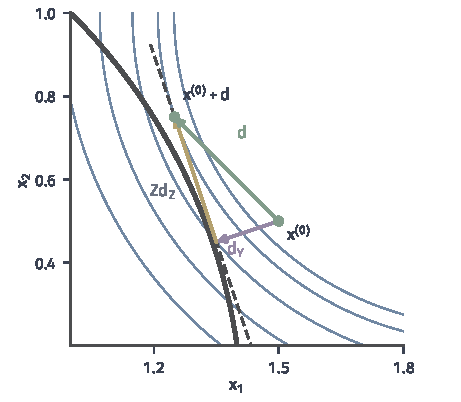
\includegraphics[width=78mm]{figures/05-optimization/06-constrained-optimization/matplotlib/sqp-range-null/figure.pdf}
 \caption{第一个局部模型的两段分解。深灰粗线是圆，虚线是线性化约束，蓝线是模型的等值线。紫色$\bm{Y}d_Y$从$\bm{x}^{(0)}$走到虚线，黄色$\bm{Z}d_Z$沿虚线走到模型的条件最小点，两段之和是绿色的$\bm{d}$。}
 \label{fig:sqp-range-null}
\end{BookInlineFigure}

\begin{BookInlineTable}
 \centering
 \begin{tabular}{lll}
  \toprule
  比较项 & 解KKT系统 & 零空间方法\\
  \midrule
  分解对象 & $(n+p)$阶对称不定 & $\bm{A}$的分解与$n-p$阶约化矩阵\\
  $n-p$很小时 & 仍解$n+p$阶 & 约化矩阵很小，便宜\\
  稀疏性 & 容易保持 & $\bm{Z}$可能变稠密\\
  检查曲率 & 需看分解的惯性 & 直接检查约化矩阵\\
  \bottomrule
 \end{tabular}
 \caption{等式QP两种解法的比较。}
 \label{tab:sqp-eqp-methods}
\end{BookInlineTable}

\paragraph{与原问题Newton步的关系}
到这里，KKT系统还只是模型的条件。现在换一个角度，从原问题出发。只含等式时，原问题的KKT条件是非线性方程组
\begin{equation}
 \bm{F}(\bm{x},\bm{\nu})=\begin{bmatrix}\nabla f(\bm{x})+\bm{A}(\bm{x})^\top\bm{\nu}\\\bm{h}(\bm{x})\end{bmatrix}=\bm{0}.
 \label{eq:sqp-kkt-map}
\end{equation}
自然的想法是对这个方程组直接用Newton法。下面的定理说，这和解局部QP是同一件事。

\begin{theorem}[SQP与KKT方程的Newton法]
\label{thm:sqp-newton}
设$\bm{B}$取Lagrange函数在$(\bm{x},\bm{\nu})$处对$\bm{x}$的Hessian。则$(\bm{\delta}_x,\bm{\delta}_\nu)$是$\bm{F}$在$(\bm{x},\bm{\nu})$处的Newton步，当且仅当$\bm{d}=\bm{\delta}_x$，$\hat{\bm{\nu}}=\bm{\nu}+\bm{\delta}_\nu$满足方程~\eqref{eq:sqp-kkt-system}。
\end{theorem}

\begin{proof}
$\bm{F}$的第一块对$\bm{x}$的导数是$\nabla^2_{\bm{x}\bm{x}}\mathcal{L}=\bm{B}$，对$\bm{\nu}$的导数是$\bm{A}^\top$；第二块对$\bm{x}$的导数是$\bm{A}$，对$\bm{\nu}$的导数为零。所以Newton方程是
\[
 \begin{bmatrix}\bm{B}&\bm{A}^\top\\\bm{A}&\bm{0}\end{bmatrix}
 \begin{bmatrix}\bm{\delta}_x\\\bm{\delta}_\nu\end{bmatrix}
 =-\begin{bmatrix}\bm{g}+\bm{A}^\top\bm{\nu}\\\bm{h}\end{bmatrix}.
\]

第一行把右端的$-\bm{A}^\top\bm{\nu}$移到左边，与$\bm{A}^\top\bm{\delta}_\nu$合并成$\bm{A}^\top(\bm{\nu}+\bm{\delta}_\nu)$，就得到方程~\eqref{eq:sqp-kkt-system}。每一步都可逆，反过来也成立。
\end{proof}

定理给出了两种读法。模型的读法是“在切平面上最小化一个二次函数”，Newton的读法是“解KKT这组方程”。前者告诉我们什么时候解是最小点，后者告诉我们为什么收敛快。两种读法也有差别：Newton法只求方程的根，不区分极小点和极大点；模型的读法多出了约化曲率这一判据。

\paragraph{计算过程}
下面把等式约束的SQP用问题~\eqref{eq:sqp-circle}完整走几轮。这里用精确的Lagrange Hessian和全步长，$\alpha^{(t)}=1$，步的接受规则留到第~\ref{sec:sqp-acceptance}节。

\needspace{6\baselineskip}
\paragraph{变量}
\begin{itemize}
 \item $\bm{x}^{(t)}\in\mathbb{R}^n$：当前点，例中$n=2$。
 \item $\bm{\nu}^{(t)}\in\mathbb{R}^p$：当前乘子估计，例中$p=1$。
 \item $\bm{g}^{(t)}\in\mathbb{R}^n$、$\bm{h}^{(t)}\in\mathbb{R}^p$：目标梯度与约束值。
 \item $\bm{A}^{(t)}\in\mathbb{R}^{p\times n}$：约束Jacobian，例中是$1\times2$的行向量。
 \item $\bm{B}^{(t)}\in\mathbb{R}^{n\times n}$：Lagrange Hessian，例中为$2\nu^{(t)}\bm{I}$。
 \item $\bm{d}^{(t)}\in\mathbb{R}^n$、$\hat{\bm{\nu}}\in\mathbb{R}^p$：子问题的解与乘子。
\end{itemize}

\paragraph{初始化}
给定$\bm{x}^{(0)}$和$\bm{\nu}^{(0)}$，以及精度$\varepsilon>0$。例中
\[
 \bm{x}^{(0)}=(1.5,\ 0.5)^\top,\qquad \nu^{(0)}=1,\qquad\varepsilon=10^{-10}.
\]

\needspace{6\baselineskip}
\paragraph{每轮更新}
\begin{enumerate}
 \item 在$\bm{x}^{(t)}$处计算$\bm{g}^{(t)},\bm{h}^{(t)},\bm{A}^{(t)}$，并由式~\eqref{eq:sqp-lagrangian-hessian}计算$\bm{B}^{(t)}$。

 例中第一轮的数值已算过。第二轮$\bm{x}^{(1)}=(1.25,0.75)^\top$，$\nu^{(1)}=0.5$，数据是
 \[
  \bm{g}^{(1)}=(-1,-1)^\top,\quad h^{(1)}=0.125,\quad\bm{A}^{(1)}=(2.5,1.5),\quad\bm{B}^{(1)}=\bm{I}.
 \]

 \item 解方程~\eqref{eq:sqp-kkt-system}得$\bm{d}^{(t)}$和$\hat{\bm{\nu}}$。$\bm{K}$可逆时，它们的显式形式是
 \begin{equation}
  \begin{bmatrix}\bm{d}^{(t)}\\\hat{\bm{\nu}}\end{bmatrix}
  =-\bigl(\bm{K}^{(t)}\bigr)^{-1}\begin{bmatrix}\bm{g}^{(t)}\\\bm{h}^{(t)}\end{bmatrix}.
  \label{eq:sqp-full-step}
 \end{equation}

 例中第一轮得$\bm{d}^{(0)}=(-0.25,0.25)^\top$，$\hat\nu=0.5$。第二轮由第一行$\bm{d}=\bm{e}-\hat\nu\bm{A}^\top$，其中$\bm{e}=(1,1)^\top$，代入第二行得
 \[
  4-8.5\,\hat\nu=-0.125,\qquad\hat\nu=\frac{33}{68}\approx0.48529.
 \]

 代回第一行，得到
 \[
  \bm{d}^{(1)}\approx(-0.21324,\ 0.27206)^\top.
 \]

 \item 更新迭代点和乘子：
 \begin{equation}
  \bm{x}^{(t+1)}=\bm{x}^{(t)}+\bm{d}^{(t)},\qquad\bm{\nu}^{(t+1)}=\hat{\bm{\nu}}.
  \label{eq:sqp-full-update}
 \end{equation}

 例中前两轮得到
 \[
  \bm{x}^{(1)}=(1.25,\ 0.75)^\top,\qquad\bm{x}^{(2)}\approx(1.03676,\ 1.02206)^\top.
 \]

 第三轮的数据是$h^{(2)}\approx0.11949$，$\bm{A}^{(2)}\approx(2.07353,2.04412)$，$\bm{B}^{(2)}\approx0.97059\,\bm{I}$，同样解方程得
 \[
  \hat\nu\approx0.49937,\qquad\bm{d}^{(2)}\approx(-0.03653,\ -0.02140)^\top.
 \]

 \item 若下面两个残差都不超过$\varepsilon$，就停止，否则回到第1步：
 \[
  \lVert\bm{g}^{(t)}+(\bm{A}^{(t)})^\top\bm{\nu}^{(t)}\rVert_2,\qquad\lVert\bm{h}^{(t)}\rVert_2.
 \]
 例中在$t=5$时停止。
\end{enumerate}

最终得到$\bm{x}^{(5)}\approx(1,1)^\top$，$\nu^{(5)}\approx0.5$。表~\ref{tab:sqp-newton-run}列出各轮结果，图~\ref{fig:sqp-newton-path}画出路径与残差。

\begin{BookInlineTable}
 \centering
 \begin{tabular}{rlllll}
  \toprule
  $t$ & $x_1^{(t)}$ & $x_2^{(t)}$ & $\nu^{(t)}$ & $\lvert h^{(t)}\rvert$ & $\lVert\bm{x}^{(t)}-\bm{x}^\star\rVert_2$\\
  \midrule
  0 & 1.5 & 0.5 & 1 & 0.5 & $7.07\times10^{-1}$\\
  1 & 1.25 & 0.75 & 0.5 & 0.125 & $3.54\times10^{-1}$\\
  2 & 1.03676 & 1.02206 & 0.48529 & 0.11949 & $4.29\times10^{-2}$\\
  3 & 1.00024 & 1.00066 & 0.49937 & $1.79\times10^{-3}$ & $7.02\times10^{-4}$\\
  4 & 1.00000 & 1.00000 & 0.50000 & $4.9\times10^{-7}$ & $4.19\times10^{-7}$\\
  5 & 1.00000 & 1.00000 & 0.50000 & $<10^{-12}$ & $2.69\times10^{-13}$\\
  \bottomrule
 \end{tabular}
 \caption{问题~\eqref{eq:sqp-circle}上全步长SQP的各轮结果。}
 \label{tab:sqp-newton-run}
\end{BookInlineTable}

\begin{BookInlineFigure}
 \centering
 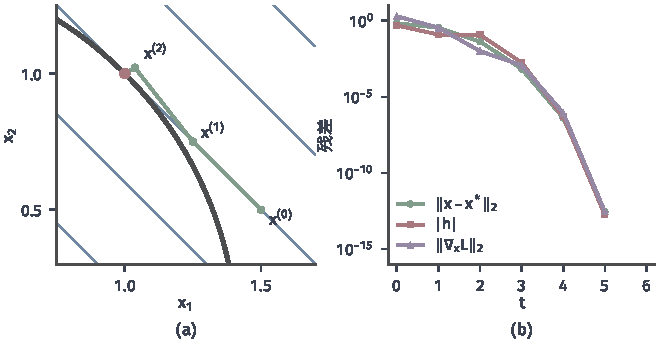
\includegraphics[width=112mm]{figures/05-optimization/06-constrained-optimization/matplotlib/sqp-newton-path/figure.pdf}
 \caption{问题~\eqref{eq:sqp-circle}上全步长SQP的运行结果。(a)~路径（绿），中间各点都不在圆上。(b)~到解的距离、约束残差和Lagrange梯度随迭代的变化，纵轴为对数，后几轮每步的有效数字大致翻倍。}
 \label{fig:sqp-newton-path}
\end{BookInlineFigure}

表中有两点值得注意。第一，约束残差的下降并不均匀，$t=1$到$t=2$几乎没有变化，因为这一步走得长，二阶误差$\lVert\bm{d}\rVert_2^2$把线性化的好处抵消了。第二，从$t=2$起误差大致平方下降，这是Newton型方法的标志，第~\ref{sec:sqp-convergence}节给出证明。

\section{有效集法（Active-Set）}
\label{sec:sqp-active-set}

等式QP一步就能解完。不等式的困难在于事先不知道解处哪些不等式取等号：如果知道，把它们当等式，其余的扔掉，就回到了上一节。接下来要弄清：怎样一边迭代、一边找出这些约束？

这就像按预算线分配资源。有些预算在最优方案中被用尽，是真正起作用的边界；有些还有富余，暂时可以当它不存在。麻烦在于，只有解出方案后才知道哪些用尽了。有效集法的做法是先猜一组，解一下，看哪里不对，再改这一组。这个类比的边界是，算法改的是它自己维护的集合，这个集合不必与当前点真实触碰的边界完全相同。

\paragraph{要解的QP}
本节讨论一个独立的QP，记号与局部模型无关，变量写作$\bm{x}$：
\begin{equation}
 \min_{\bm{x}\in\mathbb{R}^n}\ q(\bm{x})=\frac12\bm{x}^\top\bm{B}\bm{x}+\langle\bm{c},\bm{x}\rangle
 \quad\text{s.t.}\quad\langle\bm{a}_i,\bm{x}\rangle\leq b_i,\quad i=1,\ldots,m.
 \label{eq:sqp-as-qp}
\end{equation}
等式约束若有，始终留在下面要定义的集合里，写法上不必单列。全节的例子是平面上到点$\bm{c}^\circ=(4,2)^\top$的投影：
\begin{equation}
 \begin{gathered}
 q(\bm{x})=\frac12\lVert\bm{x}-\bm{c}^\circ\rVert_2^2,\\
 g_1:\ x_1+x_2\leq3,\quad g_2:\ -x_1\leq0,\quad g_3:\ -x_2\leq0,\quad g_4:\ x_1+2x_2\leq4.
 \end{gathered}
 \label{eq:sqp-as-example}
\end{equation}
它的$\bm{B}=\bm{I}$，$\bm{c}=-\bm{c}^\circ$，可行域是顶点为$(0,0),(3,0),(2,1),(0,2)$的四边形。

\paragraph{活动约束与工作集}
先把两个容易混淆的集合分开。在可行点$\bm{x}$处，取等号的约束构成\term{活动集}（active set），它由$\bm{x}$决定。算法还维护一个下标集合$\bm{W}$，这一轮把其中的约束当等式处理，它称为\term{工作集}（working set），由算法的历史决定。

可行点上工作集总是活动集的子集，但两者不必相等。图~\ref{fig:sqp-active-vs-working}给出三种情形：(a)~点贴着$g_3$的边，$g_3$活动，算法却可能没把它放进工作集；(b)~在顶点$(3,0)$处两条约束都活动，工作集可以只含其中一条；(c)~两者重合。到了解处，算法想要的是工作集恰好为那些乘子为正的约束。

\begin{BookInlineFigure}
 \centering
 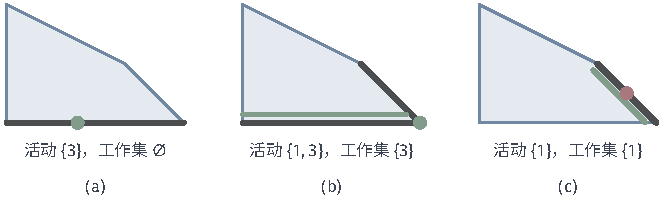
\includegraphics[width=112mm]{figures/05-optimization/06-constrained-optimization/tikz/sqp-active-vs-working/figure.pdf}
 \caption{活动集与工作集的区别，可行域取例~\eqref{eq:sqp-as-example}的四边形。深灰粗线是当前点真实触碰的边，绿色细带标出算法放进工作集的约束，圆点是当前点（红点为解）。}
 \label{fig:sqp-active-vs-working}
\end{BookInlineFigure}

\subsection{工作集的更新}
\label{sec:sqp-working-set}

本小节假设$\bm{B}\succ\bm{0}$，并且工作集中的约束梯度始终线性无关，已有一个可行的初始点。这样的初始点可以用第~\ref{chap:simplex-method}章两阶段法那样的辅助问题找到。

\paragraph{主要思想}
设$\bm{x}^{(t)}$可行，工作集为$\bm{W}$。把$\bm{W}$中的约束当等式，其余的先不管，问“从这里出发沿这张面能走到哪里”。写成对步$\bm{d}$的等式QP，并利用$\nabla q(\bm{x}^{(t)})=\bm{B}\bm{x}^{(t)}+\bm{c}$：
\begin{equation}
 \min_{\bm{d}}\ \frac12\bm{d}^\top\bm{B}\bm{d}+\langle\nabla q(\bm{x}^{(t)}),\bm{d}\rangle
 \quad\text{s.t.}\quad\langle\bm{a}_i,\bm{d}\rangle=0,\quad i\in\bm{W}.
 \label{eq:sqp-as-eqp}
\end{equation}
约束里右端是$0$，因为$\bm{W}$中的约束已经取等号，步不能破坏它们。结果分两种情况。

第一种，$\bm{d}\neq\bm{0}$。沿$\bm{d}$能降低$q$，但工作集以外的约束可能挡路。$\bm{W}$以外的约束$i$只在$\langle\bm{a}_i,\bm{d}\rangle>0$时才会变紧，走到边界所允许的比例是$(b_i-\langle\bm{a}_i,\bm{x}^{(t)}\rangle)/\langle\bm{a}_i,\bm{d}\rangle$。取其中最小的一个，并且不超过$1$，得到\term{比值检验}（ratio test）：
\begin{equation}
 \alpha^{(t)}=\min\Bigl\{1,\ \min_{i\notin\bm{W},\,\langle\bm{a}_i,\bm{d}\rangle>0}
 \frac{b_i-\langle\bm{a}_i,\bm{x}^{(t)}\rangle}{\langle\bm{a}_i,\bm{d}\rangle}\Bigr\}.
 \label{eq:sqp-ratio}
\end{equation}
新点是$\bm{x}^{(t)}$加上$\alpha^{(t)}\bm{d}$。若$\alpha^{(t)}<1$，取到最小值的约束称为\term{阻挡约束}（blocking constraint），把它加入工作集。它满足$\langle\bm{a}_b,\bm{d}\rangle>0$，而$\bm{W}$中的约束都有$\langle\bm{a}_i,\bm{d}\rangle=0$，所以它不在$\bm{W}$的约束梯度张成的子空间内，加入后仍线性无关。

第二种，$\bm{d}=\bm{0}$。当前点已是这张面上的最小点，该看乘子了。方程~\eqref{eq:sqp-kkt-system}的第一行此时给出
\begin{equation}
 \bm{B}\bm{x}^{(t)}+\bm{c}+\sum_{i\in\bm{W}}\lambda_i\bm{a}_i=\bm{0}.
 \label{eq:sqp-as-multiplier}
\end{equation}
若所有$\lambda_i\geq0$，再令$\bm{W}$以外的乘子为零，KKT条件全部成立，$\bm{B}\succ\bm{0}$时这就是全局最优解。

若有某个$\lambda_k<0$，负乘子说明这条约束不该被按住：它的影子价格是负的，相当于“放松这条预算，成本反而升高”，反过来说，向可行域内部离开这条边能让目标下降。下面的引理把这句话说准。

\begin{lemma}[释放负乘子约束]
\label{lem:sqp-drop}
设$\bm{d}=\bm{0}$时的乘子满足$\lambda_k<0$，令$\bm{W}'=\bm{W}\setminus\{k\}$，并设$\bm{d}'$是把$\bm{W}$换成$\bm{W}'$后问题~\eqref{eq:sqp-as-eqp}的解。则$\bm{d}'\neq\bm{0}$，$\bm{d}'$严格降低$q$的模型，并且
\begin{equation}
 \langle\bm{a}_k,\bm{d}'\rangle<0.
 \label{eq:sqp-drop-direction}
\end{equation}
\end{lemma}

\begin{proof}
先证$\bm{d}'\neq\bm{0}$。若$\bm{d}'=\bm{0}$，则存在系数$\mu_i$使$\nabla q+\sum_{i\in\bm{W}'}\mu_i\bm{a}_i=\bm{0}$。把它与式~\eqref{eq:sqp-as-multiplier}相减，得到$\bm{W}$中约束梯度的一个线性关系，其中$\bm{a}_k$的系数是$\lambda_k\neq0$，与线性无关矛盾。

再看方向。$\bm{d}'$的驻定条件是
\[
 \bm{B}\bm{d}'+\nabla q+\sum_{i\in\bm{W}'}\mu_i\bm{a}_i=\bm{0}.
\]

把式~\eqref{eq:sqp-as-multiplier}中的$\nabla q$代入，得
\[
 \bm{B}\bm{d}'=\sum_{i\in\bm{W}'}(\lambda_i-\mu_i)\bm{a}_i+\lambda_k\bm{a}_k.
\]

用$(\bm{d}')^\top$左乘，并注意$i\in\bm{W}'$时$\langle\bm{a}_i,\bm{d}'\rangle=0$，得到
\[
 (\bm{d}')^\top\bm{B}\bm{d}'=\lambda_k\langle\bm{a}_k,\bm{d}'\rangle.
\]
左端为正，$\lambda_k<0$，所以式~\eqref{eq:sqp-drop-direction}成立。

最后，$\bm{d}'$是等式QP的最小点而$\bm{d}=\bm{0}$可行，且最小点唯一，所以模型值严格小于零，即严格小于$\bm{d}=\bm{0}$时的模型值。
\end{proof}

式~\eqref{eq:sqp-drop-direction}的含义是，走$\bm{d}'$时被释放的约束$k$严格变松，点确实离开了这条边，不会立刻违反它。图~\ref{fig:sqp-activeset-multiplier}是例子中的这两个时刻。

\begin{BookInlineFigure}
 \centering
 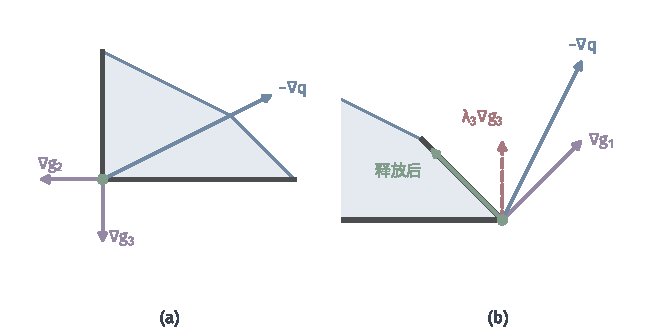
\includegraphics[width=112mm]{figures/05-optimization/06-constrained-optimization/matplotlib/sqp-activeset-multiplier/figure.pdf}
 \caption{乘子的符号。蓝色箭头是$-\nabla q$，紫色箭头是工作集约束的梯度，深灰粗线是工作集对应的边。(a)~原点处$-\nabla q=(4,2)^\top$指向可行域内部，它分解到两个向外的梯度上时系数都是负的。(b)~顶点$(3,0)^\top$处，$-\nabla q=\nabla g_1+\lambda_3\nabla g_3$，其中$\lambda_1=1$，$\lambda_3=-1$；红色虚线箭头是$\lambda_3\nabla g_3$。释放$g_3$后沿$g_1$的边（绿）走。}
 \label{fig:sqp-activeset-multiplier}
\end{BookInlineFigure}

整个逻辑可以画成图~\ref{fig:sqp-activeset-flow}。每一轮只改动工作集中的一条约束，或者加入一条，或者释放一条。

\begin{BookInlineFigure}
 \centering
 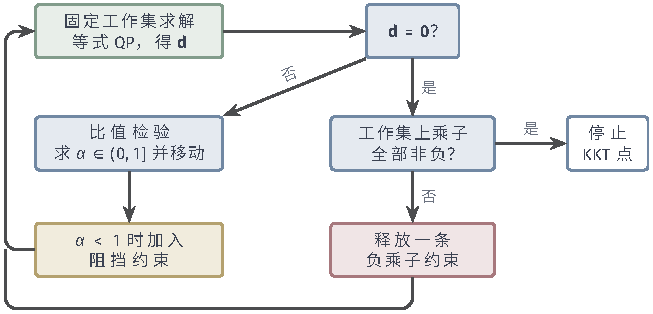
\includegraphics[width=112mm]{figures/05-optimization/06-constrained-optimization/tikz/sqp-activeset-flow/figure.pdf}
 \caption{有效集法一轮的判断。先求步；步非零则做比值检验，受阻时加入一条约束；步为零则看乘子，全部非负时停止，否则释放一条负乘子约束。}
 \label{fig:sqp-activeset-flow}
\end{BookInlineFigure}

\needspace{6\baselineskip}
\paragraph{变量}
\begin{itemize}
 \item $\bm{x}^{(t)}\in\mathbb{R}^n$：当前可行点。
 \item $\bm{W}$：工作集，下标集合，其大小不超过$n$。
 \item $\bm{A}_{\bm{W}}$：以$\bm{a}_i^\top$（$i\in\bm{W}$）为行的矩阵；$\bm{Z}_{\bm{W}}$：其零空间的基。
 \item $\bm{d}^{(t)}\in\mathbb{R}^n$：等式QP的解；$\lambda_i$（$i\in\bm{W}$）：工作集上的乘子。
\end{itemize}

\paragraph{初始化}
取可行点$\bm{x}^{(0)}$和一个工作集$\bm{W}$，其约束在$\bm{x}^{(0)}$处活动且梯度线性无关。例中取原点和它处的两条活动约束：
\[
 \bm{x}^{(0)}=(0,0)^\top,\qquad\bm{W}=\{2,3\}.
\]
目标值是$q(\bm{x}^{(0)})=10$。

\needspace{6\baselineskip}
\paragraph{每轮更新}
\begin{enumerate}
 \item 求步。由式~\eqref{eq:sqp-reduced-step}，取$\bm{h}=\bm{0}$，等式QP的解是
 \begin{equation}
  \bm{d}^{(t)}=-\bm{Z}_{\bm{W}}\bigl(\bm{Z}_{\bm{W}}^\top\bm{B}\bm{Z}_{\bm{W}}\bigr)^{-1}\bm{Z}_{\bm{W}}^\top\bigl(\bm{B}\bm{x}^{(t)}+\bm{c}\bigr).
  \label{eq:sqp-as-step}
 \end{equation}
 例中第一轮$\bm{W}=\{2,3\}$，零空间只有零向量，$\bm{d}^{(0)}=\bm{0}$。

 \item 若$\bm{d}^{(t)}=\bm{0}$，由式~\eqref{eq:sqp-as-multiplier}解出$\lambda_i$。行满秩时，用$\bm{A}_{\bm{W}}$左乘即得
 \begin{equation}
  \bm{\lambda}_{\bm{W}}=-\bigl(\bm{A}_{\bm{W}}\bm{A}_{\bm{W}}^\top\bigr)^{-1}\bm{A}_{\bm{W}}\bigl(\bm{B}\bm{x}^{(t)}+\bm{c}\bigr).
  \label{eq:sqp-as-lambda}
 \end{equation}
 全部非负就停止；否则从$\bm{W}$中去掉乘子最小的约束，令$\bm{x}^{(t+1)}=\bm{x}^{(t)}$，进入下一轮。

 例中第一轮$\nabla q=(-4,-2)^\top$，方程~\eqref{eq:sqp-as-multiplier}给出$\lambda_2=-4$，$\lambda_3=-2$。两个都是负的，释放$g_2$，得$\bm{W}=\{3\}$，$\bm{x}^{(1)}=\bm{x}^{(0)}$。

 \item 若$\bm{d}^{(t)}\neq\bm{0}$，由式~\eqref{eq:sqp-ratio}算$\alpha^{(t)}$，并移动到
 \begin{equation}
  \bm{x}^{(t+1)}=\bm{x}^{(t)}+\alpha^{(t)}\bm{d}^{(t)}.
  \label{eq:sqp-as-move}
 \end{equation}
 若$\alpha^{(t)}<1$，把阻挡约束加入$\bm{W}$。

 例中第二轮$\bm{W}=\{3\}$，$\bm{Z}_{\bm{W}}=(1,0)^\top$，由式~\eqref{eq:sqp-as-step}得$\bm{d}^{(1)}=(4,0)^\top$。比值检验只看$\langle\bm{a}_i,\bm{d}\rangle>0$的$g_1$和$g_4$：
 \[
  g_1:\ \frac{3}{4}=0.75,\qquad g_4:\ \frac{4}{4}=1.
 \]
 于是$\alpha^{(1)}=0.75$，受阻于$g_1$，得
 \[
  \bm{x}^{(2)}=(3,0)^\top,\qquad\bm{W}=\{1,3\},\qquad q(\bm{x}^{(2)})=2.5.
 \]

 第三轮零空间又只有零向量，$\bm{d}^{(2)}=\bm{0}$。此时$\nabla q=(-1,-2)^\top$，乘子满足
 \[
  \begin{bmatrix}-1\\-2\end{bmatrix}+\lambda_1\begin{bmatrix}1\\1\end{bmatrix}+\lambda_3\begin{bmatrix}0\\-1\end{bmatrix}=\bm{0}.
 \]
 第一行给$\lambda_1=1$，第二行给$\lambda_3=-1$。释放$g_3$，得$\bm{W}=\{1\}$，$\bm{x}^{(3)}=\bm{x}^{(2)}$。

 第四轮$\bm{Z}_{\bm{W}}=(1,-1)^\top$，$\bm{Z}_{\bm{W}}^\top\bm{Z}_{\bm{W}}=2$，$\bm{Z}_{\bm{W}}^\top\nabla q=1$。由式~\eqref{eq:sqp-as-step}，
 \[
  \bm{d}^{(3)}=-\frac12\begin{bmatrix}1\\-1\end{bmatrix}=(-0.5,\ 0.5)^\top.
 \]
 比值检验中$g_2$的比值是$3/0.5=6$，$g_4$的比值是$1/0.5=2$，都大于$1$，所以走满一步：
 \[
  \bm{x}^{(4)}=(2.5,\ 0.5)^\top,\qquad q(\bm{x}^{(4)})=2.25.
 \]

 \item 重复第1至3步，直到第2步发现乘子全部非负。

 例中第五轮$\bm{W}=\{1\}$，此时$\nabla q=(-1.5,-1.5)^\top$与$\bm{Z}_{\bm{W}}$正交，所以这一轮的步为零。乘子由下式确定：
 \[
  \nabla q+\lambda_1(1,1)^\top=\bm{0},\qquad\lambda_1=1.5\geq0.
 \]
 乘子非负，停止。
\end{enumerate}

最终得到$\bm{x}^\star=(2.5,0.5)^\top$，$g_1$是唯一的活动约束，影子价格$\lambda_1=1.5$。路径如图~\ref{fig:sqp-activeset-path}，每个停留的点上都发生一次工作集的变动。

\begin{BookInlineFigure}
 \centering
 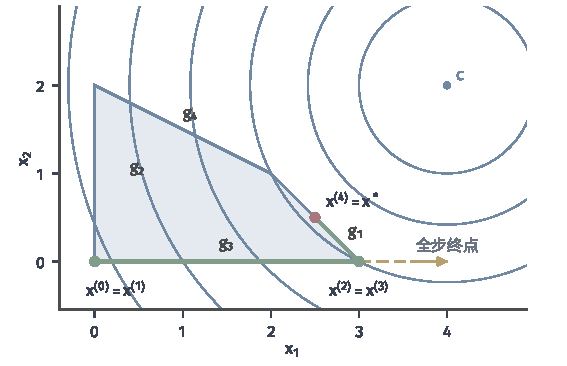
\includegraphics[width=96mm]{figures/05-optimization/06-constrained-optimization/matplotlib/sqp-activeset-path/figure.pdf}
 \caption{例~\eqref{eq:sqp-as-example}上有效集法的路径（绿）。浅蓝区域是可行域，蓝色同心圆是$q$的等高线，蓝点是无约束最小点$\bm{c}^\circ$。沿$g_3$的边本想走到$(4,0)^\top$（黄色虚线），在$(3,0)^\top$被$g_1$挡住；释放$g_3$后沿$g_1$走到红点，算法结束。}
 \label{fig:sqp-activeset-path}
\end{BookInlineFigure}

\paragraph{为什么有限步结束}
工作集的取法只有有限多种，只要同一个工作集不会被重复“解完”，算法就会停。

\begin{theorem}[有效集法的有限终止]
\label{thm:sqp-as-finite}
设$\bm{B}\succ\bm{0}$，工作集中的约束梯度始终线性无关，并且每个$\bm{d}^{(t)}\neq\bm{0}$的轮次都有$\alpha^{(t)}>0$。则算法在有限轮后停在问题~\eqref{eq:sqp-as-qp}的全局最优解。
\end{theorem}

\begin{proof}
称$\bm{d}^{(t)}=\bm{0}$的轮次为到站。两次到站之间，$\bm{W}$只增不减，所以至多有$n$轮比值检验，否则$\bm{W}$的大小超过$n$，与线性无关矛盾。由此到站必然反复发生或算法停止。

下面说明工作集不会在两次到站时重复。到站时$\bm{x}^{(t)}$是$q$在工作集约束所定义的仿射面上的唯一最小点，所以到站时的目标值由$\bm{W}$决定。

由引理~\ref{lem:sqp-drop}，到站后释放一条约束得到的步非零，严格降低模型。凸二次函数沿下降方向走$\alpha\in(0,1]$仍严格下降，而假设保证$\alpha>0$。所以相邻两次到站的目标值严格递减，同一个$\bm{W}$不会出现两次。工作集的个数有限，算法必在有限轮后到站且乘子全部非负，此时KKT条件成立，由凸性得全局最优。
\end{proof}

定理要求每次移动的步长为正。这个条件失效时会发生什么，是下面要讨论的。

\paragraph{退化、平局与热启动}
假设例中$g_4$改成$x_1+2x_2\leq3$。第二轮的比值检验中，$g_1$和$g_4$的比值都是$0.75$，出现平局，只能加入一条，另一条在下一点也活动却不在工作集中。

这一点已经是退化的：图~\ref{fig:sqp-degenerate}(b)那样，过一点的活动约束多于$n$条或梯度线性相关。这时比值检验可能算出$\alpha^{(t)}=0$，点不动，只有工作集换了一条。一连串这样的零步有可能转回原来的工作集，形成循环，定理的条件也就破坏了。

\begin{BookInlineFigure}
 \centering
 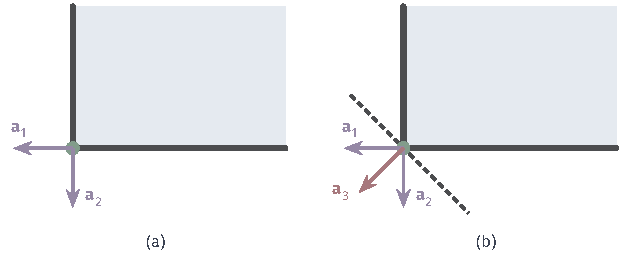
\includegraphics[width=100mm]{figures/05-optimization/06-constrained-optimization/tikz/sqp-degenerate/figure.pdf}
 \caption{顶点处的约束梯度。(a)~两条活动约束，紫色梯度线性无关，工作集的选取没有歧义。(b)~第三条约束（虚线）也经过同一点，三个梯度在平面内线性相关，工作集只能放下其中两条，走零步时点不动而工作集在变。}
 \label{fig:sqp-degenerate}
\end{BookInlineFigure}

实用的防范办法有两类。一类是确定性的选取规则，例如第~\ref{chap:simplex-method}章的Bland规则，在平局和释放时都按下标的固定顺序挑选，避免转圈。另一类是给约束右端加很小的扰动，让重合的边界分开，结束后再回到原数据上核对。释放时取最负的乘子是常用的选择，但它本身不防止循环。

有效集法还有一个明显的长处。如果手里有一个接近解的工作集，从它开始往往几轮就结束，这叫\term{热启动}（warm start）。SQP相邻两轮的QP数据只有微小变化，上一轮的工作集正是下一轮的好起点。内点法从内部出发，较难利用这种信息。每轮工作集只变一条约束，$\bm{K}$或$\bm{Z}$的分解也可以用低秩修正更新，不必重新分解。

\subsection{有效集法与SQP}
\label{sec:sqp-active-set-sqp}

把有效集法用在局部QP~\eqref{eq:sqp-qp}上时，变量是$\bm{d}$，$\bm{a}_i=\nabla g_i^{(t)}$，$b_i=-g_i^{(t)}$。本小节要回答的问题是：这样得到的工作集，和原问题解处真正活动的约束是什么关系？

\paragraph{工作集属于当前的线性化QP}
先看一个带不等式的例子，把问题~\eqref{eq:sqp-circle}的约束放宽，再加两条线性约束：
\begin{equation}
 \begin{gathered}
 \min_{\bm{x}}\ -x_1-x_2\\
 \text{s.t.}\quad g_1=x_1^2+x_2^2-2\leq0,\quad g_2=x_2-1.2\leq0,\quad g_3=-x_1\leq0.
 \end{gathered}
 \label{eq:sqp-ineq-example}
\end{equation}
解仍是$(1,1)^\top$，只有$g_1$活动，乘子$\lambda_1^\star=1/2$。下面用精确的Lagrange Hessian和全步长，从$\bm{x}^{(0)}=(0.5,1.7)^\top$、$\bm{\lambda}^{(0)}=(1,0,0)^\top$出发。

第一轮$\bm{B}^{(0)}=2\lambda_1^{(0)}\bm{I}=2\bm{I}$，约束的值和线性化约束是
\[
 \begin{gathered}
 g_1=1.14,\qquad g_2=0.5,\qquad g_3=-0.5,\\
 1.14+d_1+3.4\,d_2\leq0,\qquad 0.5+d_2\leq0,\qquad -0.5-d_1\leq0.
 \end{gathered}
\]

模型的目标是$-d_1-d_2+d_1^2+d_2^2$。先试工作集$\{2\}$：取$d_2=-0.5$，$d_1$的最优值是$0.5$。检验其余约束，线性化的$g_1$值是
\[
 1.14+0.5+3.4\times(-0.5)=-0.06\leq0,
\]
线性化的$g_3$值是$-1\leq0$，都满足。乘子由第二个驻定方程$-1+2d_2+\hat\lambda_2=0$得$\hat\lambda_2=2\geq0$。所以QP的解是
\[
 \bm{d}^{(0)}=(0.5,\ -0.5)^\top,\qquad\hat{\bm{\lambda}}=(0,\ 2,\ 0)^\top,\qquad\bm{x}^{(1)}=(1,\ 1.2)^\top.
\]

这一步说明了两件事。其一，这一轮的工作集是$\{2\}$，而原问题解处活动的是$\{1\}$：工作集属于这一轮的线性化QP，不是对原问题的最终判断。其二，$\bm{d}^{(0)}$满足全部线性化约束，新点却有
\[
 g_1(\bm{x}^{(1)})=1+1.44-2=0.44>0.
\]
QP可行不代表原问题可行，图~\ref{fig:sqp-qp-vs-nonlinear}(a)画的就是这个缺口：步落在线性化的半平面内，却冲出了圆。

\begin{BookInlineFigure}
 \centering
 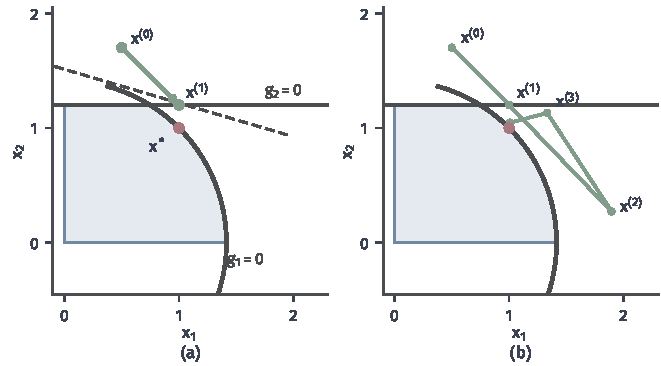
\includegraphics[width=112mm]{figures/05-optimization/06-constrained-optimization/matplotlib/sqp-qp-vs-nonlinear/figure.pdf}
 \caption{问题~\eqref{eq:sqp-ineq-example}上的SQP。浅蓝区域是真实可行域，深灰粗线是$g_1,g_2$的边界，绿色折线是迭代路径，红点是解。(a)~第一步，虚线是$g_1$在$\bm{x}^{(0)}$的线性化边界，$\bm{x}^{(1)}$满足线性化约束但在圆外。(b)~前五步的路径：工作集先后是$\{2\}$与$\{1\}$，迭代点在前几轮都不可行。}
 \label{fig:sqp-qp-vs-nonlinear}
\end{BookInlineFigure}

第二轮的乘子估计是$\lambda_1^{(1)}=0$，于是$\nabla^2_{\bm{x}\bm{x}}\mathcal{L}=\bm{0}$，子问题退化成线性规划。为了让子问题仍有曲率，这里临时取$\bm{B}^{(1)}=0.1\,\bm{I}$，这类修正下一节专门讨论。此后QP选中的工作集稳定为$\{1\}$，乘子很快接近$1/2$。图~\ref{fig:sqp-working-set-chart}列出各轮约束值和工作集。

\begin{BookInlineFigure}
 \centering
 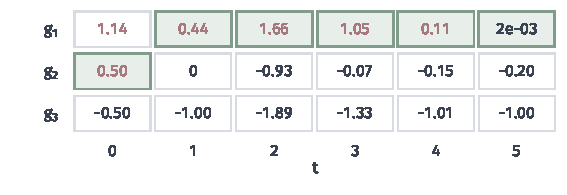
\includegraphics[width=96mm]{figures/05-optimization/06-constrained-optimization/matplotlib/sqp-working-set-chart/figure.pdf}
 \caption{问题~\eqref{eq:sqp-ineq-example}各轮的约束值$g_i(\bm{x}^{(t)})$，正值（红字）表示违反原约束，绿色格表示该约束在这一轮QP的最优工作集中。第一轮之后工作集稳定为$\{1\}$，而$g_1$的违反量要到后几轮才降下来。}
 \label{fig:sqp-working-set-chart}
\end{BookInlineFigure}

\paragraph{什么时候能认出解处的活动集}
图~\ref{fig:sqp-working-set-chart}的现象并不偶然。在解附近，QP的最优工作集会固定下来，且正好是原问题的活动集，此后的SQP就成了只含等式的SQP，上一节的结论都可以用。先复述第~\ref{chap:constrained-optimality}章的三个条件。设$(\bm{x}^\star,\bm{\lambda}^\star,\bm{\nu}^\star)$是KKT点，$\bm{S}^\star$是$\bm{x}^\star$处活动的不等式下标集。

\begin{itemize}
 \item 约束资格（LICQ）：活动不等式和全部等式的梯度在$\bm{x}^\star$处线性无关。
 \item 严格互补：对每个$i\in\bm{S}^\star$，有$\lambda_i^\star>0$。
 \item 二阶充分条件：$\nabla^2_{\bm{x}\bm{x}}\mathcal{L}$在解处沿活动约束梯度的零空间正定。在严格互补下，这就是该章临界锥上的二阶条件。
\end{itemize}

\begin{theorem}[解附近的活动集识别]
\label{thm:sqp-identification}
设上述三个条件成立。对任意有界的对称矩阵族$\{\bm{B}\}$，若它们在活动约束零空间上的约化矩阵一致正定，则存在$(\bm{x}^\star,\bm{\lambda}^\star,\bm{\nu}^\star)$的邻域，使得当当前点与乘子都在此邻域内时，QP~\eqref{eq:sqp-qp}有一个靠近$\bm{0}$的严格局部解$\bm{d}$，其活动集恰为$\bm{S}^\star$，乘子靠近$(\bm{\lambda}^\star,\bm{\nu}^\star)$。
\end{theorem}

\begin{proof}
把$\bm{S}^\star$中的不等式和全部等式都当作等式，写出方程~\eqref{eq:sqp-kkt-system}，其解记为$(\bm{d},\hat{\bm{\lambda}}_{\bm{S}^\star},\hat{\bm{\nu}})$，并令$\bm{S}^\star$以外的乘子为零。

由LICQ和约化矩阵的一致正定，KKT矩阵在该邻域内一致可逆（定理~\ref{thm:sqp-eqp}的论证与连续性）。在$(\bm{x}^\star,\bm{\lambda}^\star,\bm{\nu}^\star)$处方程右端使解为$\bm{d}=\bm{0}$，乘子为$(\bm{\lambda}^\star_{\bm{S}^\star},\bm{\nu}^\star)$。方程右端连续，而$\bm{B}\bm{d}$随$\bm{d}\to\bm{0}$趋于零，所以邻域足够小时$\bm{d}$靠近$\bm{0}$，乘子靠近其真值。

现在逐条核对条件~\eqref{eq:sqp-qp-kkt}。严格互补使$\hat\lambda_i>0$（$i\in\bm{S}^\star$），乘子符号成立。对$i\notin\bm{S}^\star$，有$g_i(\bm{x}^\star)<0$，由连续性$g_i+\langle\nabla g_i,\bm{d}\rangle<0$，这些约束严格满足。所以$\bm{d}$是QP的KKT点，活动集恰为$\bm{S}^\star$。

最后，活动约束的乘子严格为正，且$\bm{B}$在其零空间上正定，所以二阶充分条件对这个QP成立，$\bm{d}$是严格局部解。
\end{proof}

这个定理只断言“存在这样一个解”。QP非凸时可能还有别的局部解，求解器未必返回这一个；若从上一轮的工作集热启动，实际中通常就落在这一个上。条件各有其用：缺少严格互补时，$\lambda_i^\star=0$的约束可能在相邻两轮时进时出；缺少约束资格时乘子不唯一，方程组可能接近奇异。

\paragraph{原问题的检查不能省}
工作集稳定是解附近的现象，远离解时它可能频繁变动。即使稳定了，QP可行也只是切平面上的可行。所以有效集法解完子问题后，仍然要回到原问题检验新点的目标和约束，这正是第~\ref{sec:sqp-acceptance}节的内容。

\section{曲率的处理}
\label{sec:sqp-curvature}

式~\eqref{eq:sqp-lagrangian-hessian}的矩阵在解附近很好，远离解时却可能不定。这就需要回答：$\bm{B}^{(t)}$既要反映真实的局部曲率，又要让子问题有意义、让步能被接受，这两者怎样兼顾？

\paragraph{KKT系统可解不等于模型是碗}
先把两件容易混淆的事分开。设只有一条约束$d_2=0$，即$\bm{A}=(0,1)$，线性项$\bm{c}=(-0.6,0.3)^\top$，比较三个矩阵：
\[
 \bm{B}_a=\begin{bmatrix}1&0\\0&1\end{bmatrix},\qquad
 \bm{B}_b=\begin{bmatrix}1&0\\0&-1\end{bmatrix},\qquad
 \bm{B}_c=\begin{bmatrix}-1&0\\0&1\end{bmatrix}.
\]

这里零空间由$\bm{e}_1$张成，约化Hessian就是左上角的元素。三种情形下KKT矩阵都可逆，解都由$B_{1,1}d_1=0.6$给出，对应的$\bm{d}$分别是
\[
 (0.6,\ 0)^\top,\qquad(0.6,\ 0)^\top,\qquad(-0.6,\ 0)^\top.
\]

图~\ref{fig:sqp-kkt-vs-convexity}是这三个模型。情形(a)是凸的，解是最小点。情形(b)的$\bm{B}$不定，整个二次目标不是凸的，可是沿约束直线它向上弯，解仍是约束上的最小点。情形(c)的$\bm{B}$同样不定，沿直线却向下弯，解是约束上的最大点，模型沿直线无下界。

\begin{BookInlineFigure}
 \centering
 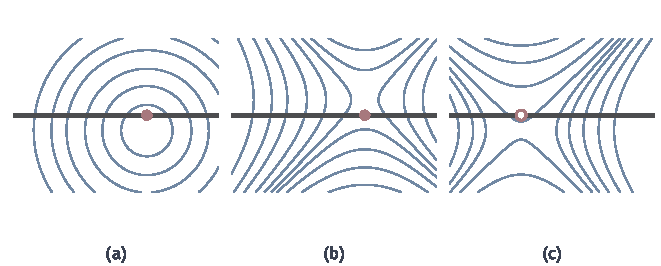
\includegraphics[width=112mm]{figures/05-optimization/06-constrained-optimization/matplotlib/sqp-kkt-vs-convexity/figure.pdf}
 \caption{三个KKT矩阵都可逆的模型，蓝线是二次目标的等高线，深灰粗线是约束$d_2=0$。(a)~$\bm{B}$正定，解（红点）是最小点。(b)~$\bm{B}$不定而约化Hessian为正，解仍是约束上的最小点。(c)~约化Hessian为负，KKT系统的解（空心点）是约束上的最大点。}
 \label{fig:sqp-kkt-vs-convexity}
\end{BookInlineFigure}

所以有三个不同的判断：KKT矩阵可逆；约化Hessian正定；$\bm{B}$在全空间正定。第三个推出第二个，第二个在行满秩时推出第一个，反过来都不成立。整个二次目标凸不凸，本身不是SQP需要的条件。

这几件事可以通过分解读出来。矩阵的\term{惯性}（inertia）是其正、负、零特征值的个数。$\bm{A}$行满秩时可以证明，$\bm{K}$的惯性等于$\bm{Z}^\top\bm{B}\bm{Z}$的惯性再各加上$p$个正、负特征值，证明要用一次合同变换，篇幅不长，读者可查阅专著\scite{math-nocedal2006numerical}。因此约化Hessian正定当且仅当$\bm{K}$恰有$n$个正特征值和$p$个负特征值。

用上面三个矩阵核对。这里$n=2$，$p=1$，$\bm{K}_a$和$\bm{K}_b$的惯性都是$(2,1,0)$；$\bm{K}_c$的特征值是$-1$和$(1\pm\sqrt5)/2$，惯性是$(1,2,0)$，多出一个负特征值，正好标记了错误的曲率。

子问题由什么方法求解，决定了实际要满足什么。表~\ref{tab:sqp-curvature-needs}按求解器列出要求。

\begin{BookInlineTable}
 \centering
 \begin{tabular}{ll}
  \toprule
  子问题的解法 & 对$\bm{B}$的实际要求\\
  \midrule
  直接解KKT系统 & 可逆即可解，是否最小点要另查惯性\\
  零空间方法 & 约化Hessian正定\\
  有效集法 & 每个工作集的约化Hessian正定\\
  要求凸QP的内点法等 & 通常要求$\bm{B}$半正定\\
  \bottomrule
 \end{tabular}
 \caption{不同子问题解法对曲率的要求。}
 \label{tab:sqp-curvature-needs}
\end{BookInlineTable}

\subsection{Hessian修正}
\label{sec:sqp-hessian-modification}

\paragraph{负曲率的例子}
乘子估计差得远时，精确的$\bm{B}$就可能是错的。回到问题~\eqref{eq:sqp-circle}的$\bm{x}^{(0)}=(1.5,0.5)^\top$，把乘子估计错成$\nu=-1$，于是$\bm{B}=2\nu\bm{I}=-2\bm{I}$，在任何方向上都向下弯。

KKT系统依然可解。第一行是$-2\bm{d}+\bm{g}+\hat\nu\bm{A}^\top=\bm{0}$，由此
\[
 \bm{d}=\frac12\bigl(\bm{g}+\hat\nu\bm{A}^\top\bigr)=\frac12\begin{bmatrix}3\hat\nu-1\\\hat\nu-1\end{bmatrix}.
\]

代入第二行$\bm{A}\bm{d}=-0.5$，左端是$5\hat\nu-2$，于是
\[
 \hat\nu=0.3,\qquad\bm{d}=(-0.05,\ -0.35)^\top.
\]

这个步是否合用，要沿线性化约束看模型。把允许的步写成$\bm{d}=\bm{d}_Y+s\bm{t}$，其中$\bm{d}_Y=(-0.15,-0.05)^\top$是第~\ref{sec:sqp-equality-qp}节的法向段，$\bm{t}=(-1,3)^\top/\sqrt{10}$是虚线的单位方向。代入模型并利用$\bm{d}_Y\perp\bm{t}$，得到
\[
 q(s)=0.175-0.632\,s-s^2.
\]

上式对$s$向下弯，模型沿线性化约束没有下界。KKT系统给出的$\bm{d}$对应$s\approx-0.316$，正是图~\ref{fig:sqp-curvature-repair}红线的最高点。求解这个方程得到的是模型的最大点，把它当作下降步是错的。

\begin{BookInlineFigure}
 \centering
 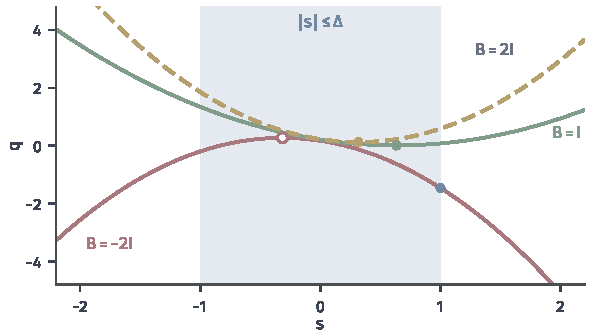
\includegraphics[width=100mm]{figures/05-optimization/06-constrained-optimization/matplotlib/sqp-curvature-repair/figure.pdf}
 \caption{沿线性化约束的模型$q(s)$，$s$是沿虚线方向的位移。红线是$\bm{B}=-2\bm{I}$，空心点是KKT系统的解，它是最大点。绿线、黄色虚线是移位后的$\bm{B}=\bm{I}$与$\bm{B}=2\bm{I}$，圆点是各自的最小点。浅蓝带是信赖域$\lvert s\rvert\leq\Delta=1$，蓝点是原模型在带内的最小点。}
 \label{fig:sqp-curvature-repair}
\end{BookInlineFigure}

\paragraph{先核对模型是否无界}
含不等式时情况稍有不同。不等式可能把下降方向挡住，QP于是有解，可是解落在边界上，是负曲率推过去的，未必是好步。所以出现负曲率时要回答两个问题：子问题本身有没有下界，以及当前这个步是否适合接受。处理的办法有三类，它们改变的东西不同。

\paragraph{移位}
第一种办法是把$\bm{B}$换成$\bm{B}+\tau\bm{I}$，这是第~\ref{chap:second-order-methods}章修正Newton法的直接推广。取$\tau$从小到大试，每次分解后检查惯性，直到约化Hessian正定。例中约化Hessian是$-2$，需要$\tau>2$。

取$\tau=3$，就是$\bm{B}=\bm{I}$。解KKT系统，第一行给$\bm{d}=(1-3\hat\nu,1-\hat\nu)^\top$，第二行给$4-10\hat\nu=-0.5$，于是
\[
 \hat\nu=0.45,\qquad\bm{d}=(-0.35,\ 0.55)^\top.
\]

移位改的是模型本身，而且改的是所有方向的曲率。$\tau$越大，步越短、越偏向梯度方向。例中$\tau=4$时步变成$(-0.25,0.25)^\top$，图~\ref{fig:sqp-curvature-repair}的黄线最低点比绿线更靠近$s=0$，就是这个效果。

\paragraph{约化曲率修正}
第二种办法只动约化Hessian。在式~\eqref{eq:sqp-reduced-step}中，把$\bm{Z}^\top\bm{B}\bm{Z}$换成一个正定矩阵，比如把负特征值取绝对值，其他量不变。例中用$\lvert-2\rvert=2$，右端不变，得到
\[
 s=\frac{0.632}{2}=0.316,\qquad\bm{d}=(-0.25,\ 0.25)^\top.
\]

这里结果恰好和$\tau=4$相同，因为$\bm{d}_Y$与$\bm{t}$正交，$\bm{B}$又是单位阵的倍数。一般两者不同：约化修正不改变法向段，也保留了$\bm{B}$在约束法方向上的信息。

\paragraph{信赖域限制}
第三种办法不改模型，而是限制步能走多远，这是第~\ref{chap:trust-region}章的想法。例中加$\lvert s\rvert\leq\Delta=1$，模型在带内的最小点在边界$s=1$，那里的模型值是$-1.457$，另一端$s=-1$的模型值是$-0.193$。

信赖域的好处是负曲率不用消除，它甚至被用来走得更远。约束优化中要多注意一件事：线性化约束和信赖域可能相互矛盾，它们的交集可能是空的。常见的处理是先取法向段，要求它只占信赖域的一部分，再在剩下的范围内取切向段。

\begin{BookInlineTable}
 \centering
 \begin{tabular}{lll}
  \toprule
  做法 & 改变了什么 & 代价或风险\\
  \midrule
  移位$\bm{B}+\tau\bm{I}$ & 所有方向的曲率 & 反复分解，步偏向梯度\\
  约化曲率修正 & 零空间内的曲率 & 需要显式的$\bm{Z}$\\
  信赖域 & 允许的步长范围 & 约束可能不相容\\
  \bottomrule
 \end{tabular}
 \caption{处理负曲率的三类办法。}
 \label{tab:sqp-modification}
\end{BookInlineTable}

这些办法各自改变了模型或步长范围。一个可解的KKT系统本身不能保证解是极小步，判断的依据只能是约化曲率或惯性。修正后的步还要经过第~\ref{sec:sqp-acceptance}节的检验。

\subsection{拟Newton近似}
\label{sec:sqp-quasi-newton}

精确的式~\eqref{eq:sqp-lagrangian-hessian}要求所有$m+p+1$个函数的二阶导数，这常常是SQP最贵也最难编写的一部分。第~\ref{chap:quasi-newton}章的办法是从梯度之差积累曲率。本小节要解决的问题是：在约束问题上，这个差该怎么取，又该怎样保持近似矩阵可用？

\paragraph{割线信息}
要近似的是Lagrange函数对$\bm{x}$的Hessian，所以差分的对象是Lagrange梯度。两点必须用同一组乘子，否则差分中混入乘子的变化，就不再是对$\nabla^2_{\bm{x}\bm{x}}\mathcal{L}$的测量。取新的乘子估计，令
\begin{equation}
 \begin{aligned}
 \bm{s}^{(t)}&=\bm{x}^{(t+1)}-\bm{x}^{(t)},\\
 \bm{y}^{(t)}&=\nabla_{\bm{x}}\mathcal{L}(\bm{x}^{(t+1)},\bm{\lambda}^{(t+1)},\bm{\nu}^{(t+1)})
 -\nabla_{\bm{x}}\mathcal{L}(\bm{x}^{(t)},\bm{\lambda}^{(t+1)},\bm{\nu}^{(t+1)}).
 \end{aligned}
 \label{eq:sqp-secant-pair}
\end{equation}

BFGS更新的公式与第~\ref{chap:quasi-newton}章相同，这里省去上标，新矩阵记作$\bm{B}^{+}$：
\begin{equation}
 \bm{B}^{+}=\bm{B}-\frac{\bm{B}\bm{s}\bm{s}^\top\bm{B}}{\bm{s}^\top\bm{B}\bm{s}}+\frac{\bm{y}\bm{y}^\top}{\bm{s}^\top\bm{y}}.
 \label{eq:sqp-bfgs}
\end{equation}

例中取第一步$\bm{s}=(-0.25,0.25)^\top$，$\hat\nu=0.5$，初始矩阵$\bm{B}=2\bm{I}$。这时Lagrange梯度是$\bm{x}-(1,1)^\top$，由它在两点之差得到
\[
 \bm{y}=\bm{s}=(-0.25,\ 0.25)^\top,\qquad\bm{s}^\top\bm{y}=0.125,\qquad\bm{s}^\top\bm{B}\bm{s}=0.25.
\]

代入式~\eqref{eq:sqp-bfgs}，并用$\bm{B}\bm{s}=2\bm{s}$，修正项化成$\bm{s}\bm{s}^\top$的倍数：
\[
 \bm{B}^{+}=2\bm{I}-16\,\bm{s}\bm{s}^\top+8\,\bm{s}\bm{s}^\top
 =\begin{bmatrix}1.5&0.5\\0.5&1.5\end{bmatrix}.
\]

可以核对割线条件$\bm{B}^{+}\bm{s}=\bm{y}$：沿$\bm{s}$的曲率从$2$变成了真实的$1$，与$\bm{s}$正交的方向仍保持$2$，因为这一次测量对那个方向没有提供信息。

\paragraph{曲率条件与阻尼}
无约束时，Wolfe线搜索能保证$\bm{s}^\top\bm{y}>0$。约束问题却不同，$\nabla^2_{\bm{x}\bm{x}}\mathcal{L}$在解处也可能是不定的，这时走出来的$\bm{s}$可能真的带着负曲率，不能靠步长选取来排除。如果$\bm{s}^\top\bm{y}\leq0$，式~\eqref{eq:sqp-bfgs}会毁掉正定性。

\term{阻尼BFGS}（damped BFGS）把$\bm{y}$换成它和$\bm{B}\bm{s}$的一个组合$\bm{r}$，组合比例只在测量不够好时才起作用：
\begin{equation}
 \begin{gathered}
 \bm{r}=\theta\bm{y}+(1-\theta)\bm{B}\bm{s},\\
 \theta=\begin{cases}
 1, & \bm{s}^\top\bm{y}\geq0.2\,\bm{s}^\top\bm{B}\bm{s},\\
 \dfrac{0.8\,\bm{s}^\top\bm{B}\bm{s}}{\bm{s}^\top\bm{B}\bm{s}-\bm{s}^\top\bm{y}}, & \text{否则}.
 \end{cases}
 \end{gathered}
 \label{eq:sqp-damped}
\end{equation}
然后在式~\eqref{eq:sqp-bfgs}中用$\bm{r}$代替$\bm{y}$。

第二种情形的$\theta$恰好使$\bm{s}^\top\bm{r}=0.2\,\bm{s}^\top\bm{B}\bm{s}>0$。把$\theta$代入即可验证：
\[
 \bm{s}^\top\bm{r}=\bm{s}^\top\bm{B}\bm{s}+\theta\bigl(\bm{s}^\top\bm{y}-\bm{s}^\top\bm{B}\bm{s}\bigr)=\bm{s}^\top\bm{B}\bm{s}-0.8\,\bm{s}^\top\bm{B}\bm{s}.
\]

所以更新后的矩阵总保持正定。图~\ref{fig:sqp-damped-rule}按上例的$\bm{s}^\top\bm{B}\bm{s}=0.25$画出这条规则。设乘子为负，真实曲率是$-2$，即$\bm{y}=-2\bm{s}$，$\bm{s}^\top\bm{y}=-0.25$，于是
\[
 \theta=\frac{0.8\times0.25}{0.25+0.25}=0.4,\qquad\bm{r}=0.4\bm{s}.
\]

沿$\bm{s}$的曲率更新后是$0.05/0.125=0.4$，即$\bm{s}^\top\bm{r}$除以$\bm{s}^\top\bm{s}$。它既不是测量到的$-2$，也不是原来的$2$。阻尼的代价是割线条件不再成立，矩阵不再记录真实的负曲率。

\begin{BookInlineFigure}
 \centering
 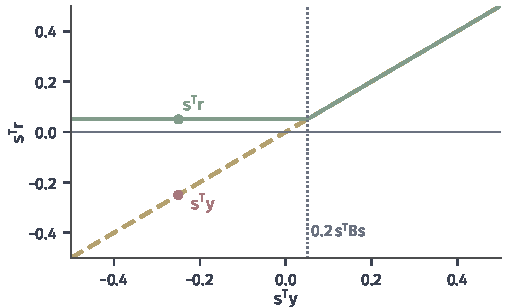
\includegraphics[width=86mm]{figures/05-optimization/06-constrained-optimization/matplotlib/sqp-damped-rule/figure.pdf}
 \caption{阻尼规则，$\bm{s}^\top\bm{B}\bm{s}=0.25$。黄色虚线是未加处理的$\bm{s}^\top\bm{y}$，绿线是阻尼后的$\bm{s}^\top\bm{r}$，它在虚线竖线以左被托在$0.2\,\bm{s}^\top\bm{B}\bm{s}=0.05$。红点是测量值$-0.25$，绿点是阻尼后的$0.05$。}
 \label{fig:sqp-damped-rule}
\end{BookInlineFigure}

\paragraph{成本与速度}
下面比较两种选择。精确Hessian每轮要算$m+p+1$个Hessian，但步是Newton型的，轮数少。拟Newton只需要梯度，却维护一个稠密的$n\times n$矩阵，破坏了$\bm{K}$可能具有的稀疏结构，这时可以改用有限记忆的表示。

图~\ref{fig:sqp-exact-bfgs-rate}是一个五变量问题上的比较，目标与约束为
\[
 \begin{gathered}
 f=\exp(x_1x_2x_3x_4x_5)-\tfrac12(x_1^3+x_2^3+1)^2,\\
 h_1=\lVert\bm{x}\rVert_2^2-10,\quad h_2=x_2x_3-5x_4x_5,\quad h_3=x_1^3+x_2^3+1.
 \end{gathered}
\]
从$(-1.8,1.7,1.9,-0.8,-0.8)^\top$与最小二乘乘子出发，精确Hessian的全步法$4$轮将误差降到$10^{-11}$以下；阻尼BFGS（$\bm{B}^{(0)}=\bm{I}$，罚函数回溯，第~\ref{sec:sqp-merit}节）前$18$轮都在攒曲率信息，步长常被缩短，之后几轮迅速下降，共需约$21$轮。

\begin{BookInlineFigure}
 \centering
 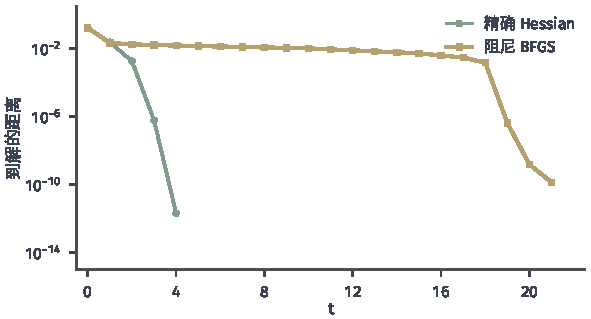
\includegraphics[width=100mm]{figures/05-optimization/06-constrained-optimization/matplotlib/sqp-exact-bfgs-rate/figure.pdf}
 \caption{五变量问题上到解的距离。绿线是精确Lagrange Hessian的全步长SQP，黄线是阻尼BFGS加罚函数回溯。两者起点相同，后者每轮不需要二阶导数。}
 \label{fig:sqp-exact-bfgs-rate}
\end{BookInlineFigure}

这个对比只是一个例子，轮数的差距随问题而变。局部速度的结论还需要曲率近似的条件。记$\bm{P}^{(t)}$是向$\bm{A}^{(t)}$零空间的投影，$\bm{H}_{\mathcal{L}}^\star$是Lagrange函数在解处对$\bm{x}$的Hessian，需要的条件是
\begin{equation}
 \lim_{t\to\infty}\frac{\lVert\bm{P}^{(t)}\bigl(\bm{B}^{(t)}-\bm{H}_{\mathcal{L}}^\star\bigr)\bm{d}^{(t)}\rVert_2}{\lVert\bm{d}^{(t)}\rVert_2}=0.
 \label{eq:sqp-dennis-more}
\end{equation}
它只要求沿步的方向、在切空间内近似准确，不要求$\bm{B}^{(t)}$收敛到真实的Hessian。这一点很重要，因为$\bm{H}_{\mathcal{L}}^\star$可以不定，而正定的BFGS矩阵无法趋于不定矩阵；在切空间上$\bm{H}_{\mathcal{L}}^\star$却是正定的，式~\eqref{eq:sqp-dennis-more}仍可能成立。

\section{更新的接受}
\label{sec:sqp-acceptance}

QP给出的步只在模型里是好的。把步放回非线性问题，凭什么判断它值得采用？

无约束时这个问题很简单，看目标有没有下降。约束问题有两个指标。第~\ref{sec:sqp-equality-qp}节的第三步目标从$-2.0588$升到$-2.0009$，约束违反却从$0.119$降到$0.0018$；而从圆上的点$(1.4,0.2)^\top$走一个全步，目标从$-1.6$降到$-2.32$，违反量却从$0$升到$0.72$。两个指标常常冲突，必须有一条明确规则来评价进展。第~\ref{sec:sqp-merit}小节把两者压成一个数，第~\ref{sec:sqp-filter}小节把两者并排比较。

记约束的总违反量为
\begin{equation}
 \theta(\bm{x})=\sum_{j=1}^p\lvert h_j(\bm{x})\rvert+\sum_{i=1}^m[g_i(\bm{x})]_+,
 \label{eq:sqp-violation}
\end{equation}
其中$[u]_+=\max\{u,0\}$。

\subsection{罚函数线搜索}
\label{sec:sqp-merit}

\paragraph{评价函数}
把目标和违反量加起来，用一个权重$\rho>0$换算两者的单位，得到
\begin{equation}
 \phi_\rho(\bm{x})=f(\bm{x})+\rho\,\theta(\bm{x}).
 \label{eq:sqp-merit}
\end{equation}
这是第~\ref{chap:penalty-multiplier-methods}章的$\ell_1$精确惩罚函数，在这里它的角色是判断步的好坏，称为\term{评价函数}（merit function）。那一章的结论是：若$\bm{x}^\star$满足二阶充分条件，且权重大于乘子的最大绝对值，则$\bm{x}^\star$是$\phi_\rho$的严格局部最小点。乘子是约束的影子价格，权重就是愿意为单位违反付的罚款，罚款低于影子价格，违约反而划算。

$\phi_\rho$在$h_j=0$或$g_i=0$处不可微，但沿任意方向的方向导数存在。记$D(\phi_\rho;\bm{d})$为它在$\bm{x}^{(t)}$处沿$\bm{d}$的方向导数。下面的引理告诉我们，QP的解在什么时候是下降方向。

\begin{lemma}[QP步的下降性]
\label{lem:sqp-merit-descent}
设$(\bm{d},\hat{\bm{\lambda}},\hat{\bm{\nu}})$满足条件~\eqref{eq:sqp-qp-kkt}，则
\begin{equation}
 D(\phi_\rho;\bm{d})\leq-\bm{d}^\top\bm{B}^{(t)}\bm{d}-\bigl(\rho-\max\{\lVert\hat{\bm{\nu}}\rVert_\infty,\lVert\hat{\bm{\lambda}}\rVert_\infty\}\bigr)\theta(\bm{x}^{(t)}).
 \label{eq:sqp-merit-descent}
\end{equation}
\end{lemma}

\begin{proof}
分别计算$\theta$和$f$的方向导数。先看等式项。线性化约束给出$\langle\nabla h_j,\bm{d}\rangle=-h_j$。若$h_j\neq0$，则$\lvert h_j\rvert$的方向导数是$h_j$的符号乘以$\langle\nabla h_j,\bm{d}\rangle$，等于$-\lvert h_j\rvert$；若$h_j=0$，则$\langle\nabla h_j,\bm{d}\rangle=0$，方向导数为$0$。两种情况都等于$-\lvert h_j\rvert$。

再看不等式项，线性化约束给出$\langle\nabla g_i,\bm{d}\rangle\leq-g_i$。若$g_i>0$，$[g_i]_+$的方向导数是$\langle\nabla g_i,\bm{d}\rangle\leq-[g_i]_+$；若$g_i=0$，方向导数是$[\langle\nabla g_i,\bm{d}\rangle]_+=0$；若$g_i<0$，方向导数是$0$。三种情况都不超过$-[g_i]_+$。把这些加起来，得到
\[
 D(\theta;\bm{d})\leq-\theta(\bm{x}^{(t)}).
\]

然后看目标。用$\bm{d}^\top$左乘式~\eqref{eq:sqp-qp-kkt}第一行，再用线性化约束和互补条件换掉$\bm{A}\bm{d}$和$\bm{G}\bm{d}$：
\[
 \begin{aligned}
 \langle\nabla f,\bm{d}\rangle
 &=-\bm{d}^\top\bm{B}\bm{d}-\hat{\bm{\nu}}^\top\bm{A}\bm{d}-\hat{\bm{\lambda}}^\top\bm{G}\bm{d}\\
 &=-\bm{d}^\top\bm{B}\bm{d}+\hat{\bm{\nu}}^\top\bm{h}+\hat{\bm{\lambda}}^\top\bm{g}.
 \end{aligned}
\]

最后估计两个内积。第一个用Hölder不等式，第二个先用$\hat{\bm{\lambda}}\geq\bm{0}$把$\bm{g}$放大成$[\bm{g}]_+$，再用Hölder不等式：
\[
 \begin{aligned}
 \hat{\bm{\nu}}^\top\bm{h}&\leq\lVert\hat{\bm{\nu}}\rVert_\infty\lVert\bm{h}\rVert_1,\\
 \hat{\bm{\lambda}}^\top\bm{g}&\leq\hat{\bm{\lambda}}^\top[\bm{g}]_+\leq\lVert\hat{\bm{\lambda}}\rVert_\infty\lVert[\bm{g}]_+\rVert_1.
 \end{aligned}
\]

合起来，
\[
 \langle\nabla f,\bm{d}\rangle\leq-\bm{d}^\top\bm{B}\bm{d}+\max\{\lVert\hat{\bm{\nu}}\rVert_\infty,\lVert\hat{\bm{\lambda}}\rVert_\infty\}\,\theta(\bm{x}^{(t)}).
\]
$\phi_\rho$的方向导数是$\langle\nabla f,\bm{d}\rangle$与$\rho D(\theta;\bm{d})$之和，式~\eqref{eq:sqp-merit-descent}成立。
\end{proof}

引理说明，当$\rho$超过QP乘子的最大绝对值，并且$\bm{d}^\top\bm{B}\bm{d}$为正时，$\bm{d}$是$\phi_\rho$的下降方向。这里的正性只需在$\bm{d}$上成立。$\bm{d}^\top\bm{B}\bm{d}$可能为负时，条件要通过第~\ref{sec:sqp-curvature}节的修正来保证。

\paragraph{权重的两难}
式~\eqref{eq:sqp-merit-descent}要求$\rho$足够大，但$\rho$并不是越大越好。看问题~\eqref{eq:sqp-circle}沿射线$x_1=x_2=s$的情形，此时
\[
 \phi_\rho(s,s)=-2s+\rho\,\lvert2s^2-2\rvert.
\]

在$s>1$上，$\phi_\rho$的导数是$-2+4\rho s$。$\rho=0.1$时导数在$s=5$才变号，评价函数在$(5,5)$有局部最小值，其值$-5.2$比解处的$-2$还小。沿着$\phi_{0.1}$下降会被带到严重违约的地方。

$s=1$处的右导数是$-2+4\rho$，要它为正需要$\rho>1/2=\nu^\star$，这正是权重要超过乘子的具体含义。图~\ref{fig:sqp-merit-rho-ray}比较了三种权重。权重过大时，$\phi_\rho$在约束面两侧形成很陡的峡谷，任何离开约束面的步，即使只离开$\lVert\bm{d}\rVert_2^2$这么多，也要付很高的代价，步长于是被压得很小，迭代只能贴着约束面慢慢挪。

\begin{BookInlineFigure}
 \centering
 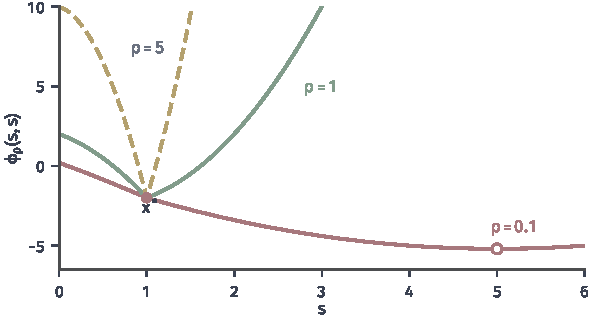
\includegraphics[width=100mm]{figures/05-optimization/06-constrained-optimization/matplotlib/sqp-merit-rho-ray/figure.pdf}
 \caption{评价函数沿射线$x_1=x_2=s$的形状。红线$\rho=0.1$低于乘子，空心点$(5,5)$是错误的局部最小点；绿线$\rho=1$在解$s=1$（红点）处形成拐点；黄色虚线$\rho=5$的峡谷很陡。}
 \label{fig:sqp-merit-rho-ray}
\end{BookInlineFigure}

实际算法动态调整权重。常用规则是每轮令$\rho$不小于当前QP乘子的最大绝对值再加一个裕量$\delta>0$：
\begin{equation}
 \rho^{(t)}\geq\max\{\lVert\hat{\bm{\nu}}\rVert_\infty,\lVert\hat{\bm{\lambda}}\rVert_\infty\}+\delta.
 \label{eq:sqp-rho-rule}
\end{equation}
权重只升不降时，迭代的后期可能一直背着远离解时抬高的权重，因此实现中也允许有控制地下调。

\paragraph{主要思想}
有了下降方向，就和无约束问题一样回溯。从$\alpha=1$开始试，直到满足充分下降条件：
\begin{equation}
 \phi_\rho(\bm{x}^{(t)}+\alpha\bm{d}^{(t)})\leq\phi_\rho(\bm{x}^{(t)})+\eta\,\alpha\,D(\phi_\rho;\bm{d}^{(t)}),
 \label{eq:sqp-armijo}
\end{equation}
其中$\eta\in(0,1/2)$。由于$\phi_\rho$沿$\bm{d}$在$\alpha=0$右侧的导数就是$D$，小的$\alpha$总能满足这个条件。

\needspace{6\baselineskip}
\paragraph{变量}
\begin{itemize}
 \item $\bm{x}^{(t)}$、$\bm{\nu}^{(t)}$：当前点与乘子；$\rho$：评价函数的权重。
 \item $\bm{d}^{(t)}$、$\hat{\bm{\nu}}$：QP的解与乘子；$D$：$\phi_\rho$的方向导数。
 \item $\eta$：充分下降系数；$\alpha^{(t)}$：接受的步长。
\end{itemize}

\paragraph{初始化}
给定$\bm{x}^{(0)}$、$\bm{\nu}^{(0)}$、$\rho$和$\eta$。例中取圆上的一点，数据是
\[
 \bm{x}^{(0)}=(1.4,\ 0.2)^\top,\qquad\nu^{(0)}=0.5,\qquad\rho=2,\qquad\eta=0.1.
\]
这里$h(\bm{x}^{(0)})=1.96+0.04-2=0$，点是可行的，$\phi_\rho(\bm{x}^{(0)})=-1.6$。

\needspace{6\baselineskip}
\paragraph{每轮更新}
\begin{enumerate}
 \item 解QP得$\bm{d}^{(t)}$和乘子。例中第一轮$\bm{B}=\bm{I}$，$\bm{A}=(2.8,0.4)$，$h=0$，解得
 \[
  \hat\nu=0.4,\qquad\bm{d}^{(0)}=(-0.12,\ 0.84)^\top.
 \]

 \item 按需要增大$\rho$，并计算方向导数，即$D=\langle\nabla f,\bm{d}\rangle-\rho\,\theta$（只含等式时）。例中$\rho=2\geq\hat\nu$，$\theta=0$，于是
 \[
  D=\langle(-1,-1)^\top,\bm{d}^{(0)}\rangle=-0.72.
 \]

 \item 令$\alpha=1$，当式~\eqref{eq:sqp-armijo}不成立时令$\alpha\leftarrow\alpha/2$。例中沿$\bm{d}$有$h(\bm{x}+\alpha\bm{d})=0.72\alpha^2$，$f(\bm{x}+\alpha\bm{d})=-1.6-0.72\alpha$，所以
 \[
  \phi_\rho(\alpha)=-1.6-0.72\,\alpha+1.44\,\alpha^2.
 \]

 依次试三个步长，每个步长下左边是$\phi_\rho$的值，右边是式~\eqref{eq:sqp-armijo}的门槛：
 \[
  \begin{aligned}
  \alpha=1:&\quad-0.88>-1.672,\\
  \alpha=0.5:&\quad-1.6>-1.636,\\
  \alpha=0.25:&\quad-1.69\leq-1.618.
  \end{aligned}
 \]
 前两个被拒绝，第三个被接受，图~\ref{fig:sqp-merit-armijo}画出了这三次试探。

 \item 更新迭代点，乘子按式~\eqref{eq:sqp-multiplier-update}。例中第一轮
 \[
  \bm{x}^{(1)}=(1.37,\ 0.41)^\top,\qquad\nu^{(1)}=0.5+0.25\,(0.4-0.5)=0.475.
 \]

 第二轮$h=0.045$，$\bm{d}^{(1)}\approx(-0.21767,0.67247)^\top$，$\alpha^{(1)}=0.25$；第三轮$\alpha^{(2)}=0.5$；第四轮起$\alpha^{(t)}=1$。

 \item 按第~\ref{sec:sqp-convergence}节的残差判断是否停止。
\end{enumerate}

最终$\bm{x}^{(t)}$到达$(1,1)^\top$，例中$t=6$时到解的距离已低于$10^{-6}$。

\begin{BookInlineFigure}
 \centering
 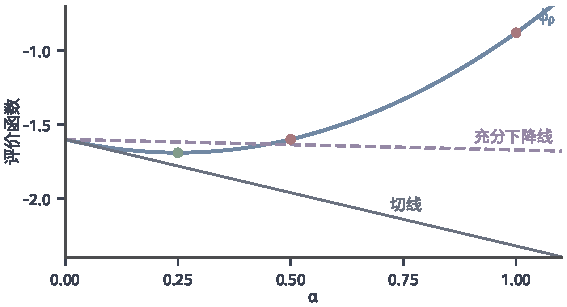
\includegraphics[width=96mm]{figures/05-optimization/06-constrained-optimization/matplotlib/sqp-merit-armijo/figure.pdf}
 \caption{从$\bm{x}^{(0)}=(1.4,0.2)^\top$沿QP步的评价函数，$\rho=2$。蓝线是$\phi_\rho(\alpha)$，灰线是切线，紫色虚线是充分下降的门槛。红点$\alpha=1$与$\alpha=0.5$被拒绝，绿点$\alpha=0.25$被接受。}
 \label{fig:sqp-merit-armijo}
\end{BookInlineFigure}

这个例子还暗示了一个毛病。全步到达$(1.28,1.04)^\top$，到解的距离从$0.894$缩到$0.283$，明明很好，评价函数却把它拒绝了。原因及补救在第~\ref{sec:sqp-soc}小节。

\paragraph{用信赖域代替线搜索}
线搜索固定方向、调整步长。也可以用第~\ref{chap:trust-region}章的方式固定一个半径，比较实际下降与模型预测，比值大则接受并放大半径，比值小则缩小半径。线性化的约束有可能与半径冲突，所以需要第~\ref{sec:sqp-hessian-modification}小节提到的法向段与切向段的安排。信赖域版本可以自然处理负曲率，代价是实现更复杂。

\subsection{过滤器}
\label{sec:sqp-filter}

罚函数要预先定一个换算比例。本小节要回答的问题是：能不能不做这个换算，直接比较$\theta$和$f$这两个指标？

\paragraph{基本想法}
类比两人比赛：如果候选步在两个指标上都比某个历史记录差，就没有接受的理由；只要在某个指标上比所有记录都更好，就给它一个机会。把已接受的点的$(\theta,f)$对存下来，这个集合称为\term{过滤器}（filter），记为$\mathcal{F}$。

如果只要求“不被支配”，也就是不被某条记录在两个指标上同时压过，算法可能无限地取得微不足道的进步。设想$\theta$的序列是$1+1/k$，每一项都比前一项略小，$f$保持不变，每一步都不被支配，极限却是$\theta=1$，一个不可行的点。所以真正的条件要带裕量。

\begin{definition}[过滤器的接受条件]
\label{def:sqp-filter}
给定$\gamma\in(0,1)$，候选点$\bm{x}^{+}$可被过滤器$\mathcal{F}$接受，是指对每条记录$(\theta_l,f_l)\in\mathcal{F}$，都有
\begin{equation}
 \theta(\bm{x}^{+})\leq(1-\gamma)\,\theta_l\quad\text{或}\quad f(\bm{x}^{+})\leq f_l-\gamma\,\theta_l.
 \label{eq:sqp-filter}
\end{equation}
\end{definition}

条件的后半式里的裕量是$\gamma\theta_l$，它与违反量成比例。这样一来，要么约束违反按比例减小，要么目标确实下降一段距离，前面那个微小进步的序列不再能被接受。

用一组教学数据演示。取$\gamma=0.1$，三条记录为
\[
 (\theta_1,f_1)=(0.8,-2.6),\quad(\theta_2,f_2)=(0.3,-2.2),\quad(\theta_3,f_3)=(0.05,-1.9).
\]

候选点$A=(0.2,-2.4)$：对记录一，$0.2\leq0.72$；对记录二，$0.2\leq0.27$；对记录三，$\theta$不够小，但目标满足$-2.4\leq-1.905$。三条都通过，接受。

候选点$B=(0.4,-2.0)$：对记录一通过；对记录二，$0.4>0.27$，目标$-2.0>-2.23$，失败，拒绝。

候选点$C=(0.295,-2.205)$看上去比记录二好一点，$\theta$和$f$都略小。但$0.295>0.27$，$-2.205>-2.23$，改进不够裕量，同样拒绝。图~\ref{fig:sqp-filter-plane}是这三个点的位置。

\begin{BookInlineFigure}
 \centering
 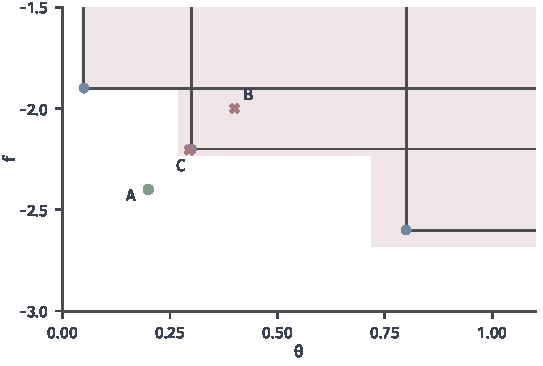
\includegraphics[width=92mm]{figures/05-optimization/06-constrained-optimization/matplotlib/sqp-filter-plane/figure.pdf}
 \caption{过滤器的$(\theta,f)$平面，蓝点是三条记录，深灰线是它们支配的范围边界，红色浅底是带裕量$\gamma=0.1$的禁止区。绿点$A$被接受，红叉$B$和$C$被拒绝，其中$C$虽不被支配，但在裕量带内。}
 \label{fig:sqp-filter-plane}
\end{BookInlineFigure}

\paragraph{还需要什么}
只靠式~\eqref{eq:sqp-filter}并不足以保证收敛到KKT点。还要回答三件事。

第一，局部切换。若迭代点已经几乎可行，而模型预测目标有明显下降，就不能只凭$\theta$有所改善就接受，要转而要求目标满足类似式~\eqref{eq:sqp-armijo}的充分下降，这样的步也不写入过滤器。否则算法可能收敛到一个可行但并不最优的点。

第二，什么时候写入记录。不满足上述切换条件而被接受的步，把当前点的$(\theta,f)$写入过滤器，并删去被它支配的旧记录。这样禁止区只会扩大，同一区域不会被反复光顾。

第三，可行性恢复。回溯到很小的步长仍无法被接受，说明当前的线性化方向帮不上忙，这时转入下一节的恢复阶段。过滤器不能代替这些规则。

表~\ref{tab:sqp-merit-filter}总结了两种规则。

\begin{BookInlineTable}
 \centering
 \begin{tabular}{lll}
  \toprule
  比较项 & 罚函数 & 过滤器\\
  \midrule
  进展的度量 & 一个数$\phi_\rho$ & 两个数$(\theta,f)$\\
  需要的参数 & 权重$\rho$ & 裕量$\gamma$、切换常数\\
  主要风险 & $\rho$太小或太大 & 需额外的恢复与切换\\
  历史信息 & 不保存 & 保存记录\\
  \bottomrule
 \end{tabular}
 \caption{罚函数线搜索与过滤器的比较。}
 \label{tab:sqp-merit-filter}
\end{BookInlineTable}

\section{模型的修复}
\label{sec:sqp-repair}

前面两节都假定子问题有解，候选步也还算合用。本节处理两种不成立的情形，要回答的问题是：失败发生在哪一层，相应地该修什么？第一种失败发生在子问题上，线性化约束根本没有可行解，此时缩小步长毫无用处，因为连可以缩小的步都不存在。第二种失败发生在候选步上，QP有解，步却被真实约束的弯曲挡住。

图~\ref{fig:sqp-repair-tree}按失败原因列出修复手段。只靠反复缩小步长处理所有问题，第一种情形无效，第二种情形则会拖慢收敛。

\begin{BookInlineFigure}
 \centering
 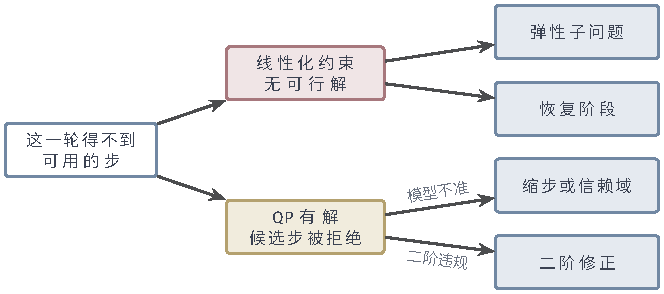
\includegraphics[width=112mm]{figures/05-optimization/06-constrained-optimization/tikz/sqp-repair-tree/figure.pdf}
 \caption{得不到可用的步时的两类原因及其修复。红框是子问题层面的失败，黄框是候选步层面的失败，蓝框是对应的处理。}
 \label{fig:sqp-repair-tree}
\end{BookInlineFigure}

\subsection{可行性恢复}
\label{sec:sqp-restoration}

\paragraph{线性化约束可能相互矛盾}
原问题可行，并不意味着它的线性化可行。看下面的问题：
\begin{equation}
 \min_{\bm{x}}\ \frac12\bigl((x_1-2)^2+x_2^2\bigr)
 \quad\text{s.t.}\quad h_1=x_2-x_1^2=0,\quad h_2=x_2-1=0.
 \label{eq:sqp-inconsistent}
\end{equation}
可行点只有$(\pm1,1)^\top$，解是$\bm{x}^\star=(1,1)^\top$。从原点出发，约束的值和Jacobian是
\[
 \bm{h}^{(0)}=(0,-1)^\top,\qquad\bm{A}^{(0)}=\begin{bmatrix}0&1\\0&1\end{bmatrix}.
\]

线性化约束成为$d_2=0$和$d_2=1$，两者矛盾。抛物线在顶点的切线是水平的，与直线$x_2=1$平行，图~\ref{fig:sqp-inconsistent}(a)里两条线永不相交。这里$\bm{A}^{(0)}$的秩为$1$，定理~\ref{thm:sqp-eqp}的前提失效。

\begin{BookInlineFigure}
 \centering
 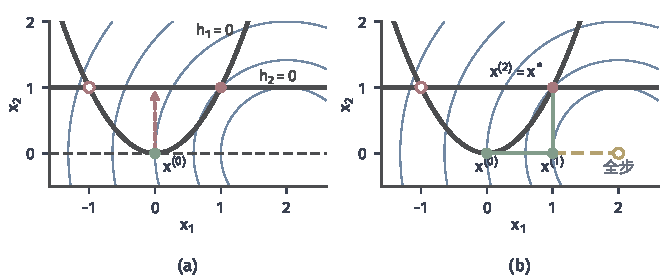
\includegraphics[width=112mm]{figures/05-optimization/06-constrained-optimization/matplotlib/sqp-inconsistent/figure.pdf}
 \caption{问题~\eqref{eq:sqp-inconsistent}。深灰粗线是抛物线$h_1=0$和直线$h_2=0$，蓝线是目标的等高线，红点是解，空心点是另一个可行点。(a)~原点处抛物线的线性化（虚线）与$h_2=0$平行，红色箭头表示两者之间的距离无法消除。(b)~弹性子问题的全步到$(2,0)^\top$（黄色虚线），回溯到一半得$\bm{x}^{(1)}$，下一轮的QP相容，一步到解。}
 \label{fig:sqp-inconsistent}
\end{BookInlineFigure}

\paragraph{弹性子问题}
第一种修复是让约束可以有偿违反。给每条线性化约束加上非负的松弛变量，并在目标中按权重$\rho$收费，得到\term{弹性子问题}（elastic subproblem）：
\begin{equation}
 \begin{aligned}
 \min_{\bm{d},\bm{v},\bm{w},\bm{u}}\quad & \langle\nabla f,\bm{d}\rangle+\frac12\bm{d}^\top\bm{B}\bm{d}
 +\rho\bigl(\langle\bm{1},\bm{v}+\bm{w}\rangle+\langle\bm{1},\bm{u}\rangle\bigr)\\
 \text{s.t.}\quad & \bm{h}+\bm{A}\bm{d}=\bm{v}-\bm{w},\\
 & \bm{g}+\bm{G}\bm{d}\leq\bm{u},\\
 & \bm{v},\bm{w},\bm{u}\geq\bm{0}.
 \end{aligned}
 \label{eq:sqp-elastic}
\end{equation}
它对任何数据都可行，取$\bm{d}=\bm{0}$，松弛变量等于当前的违反量即可。

消去松弛变量，式~\eqref{eq:sqp-elastic}就是在线性化约束上最小化$\ell_1$惩罚的模型。第~\ref{chap:penalty-multiplier-methods}章的精确惩罚论证用在这个凸QP上，得到：当线性化约束相容且$\rho$大于QP乘子的最大绝对值时，松弛变量全为零，弹性解就是原来QP的解。所以可以总是求解弹性形式，不必先判断QP是否可行。

例中取$\bm{B}^{(0)}=\bm{I}$，$\rho=1$。$\nabla f=(-2,0)^\top$，消去松弛变量后，模型是
\[
 -2d_1+\frac12d_1^2+\frac12d_2^2+\lvert d_2\rvert+\lvert d_2-1\rvert.
\]

对$d_1$的最小化独立于$d_2$，得$d_1=2$。在$0\leq d_2\leq1$上两个绝对值之和恒为$1$，这个区间内只剩$\frac12d_2^2$起作用，所以$d_2=0$。于是
\[
 \bm{d}^{(0)}=(2,\ 0)^\top,\qquad\text{模型中的违反量}=1.
\]

这一步并没有修好$h_2$，只是把目标朝$x_1$方向推。候选点要用真实函数检验。起点的评价函数是$\phi_1(\bm{0})=2+1=3$，全步的值和半步的值分别是
\[
 \phi_1(2,0)=0+4+1=5,\qquad\phi_1(1,0)=0.5+1+1=2.5.
\]

全步因线性化高估而被拒绝，半步通过。于是$\bm{x}^{(1)}=(1,0)^\top$。这里$h_1=-1$，梯度变成$(-2,1)$，第一行不再与第二行平行，线性化约束变成
\[
 -1-2d_1+d_2=0,\qquad-1+d_2=0.
\]

它有唯一解$\bm{d}^{(1)}=(0,1)^\top$，下一点恰好就是$(1,1)^\top$。这里能一步到解有偶然的成分，两个约束两个变量，线性化解恰好落在抛物线上。要点是离开奇异点之后，线性化又恢复了相容，图~\ref{fig:sqp-inconsistent}(b)是这条路径。

\paragraph{恢复阶段}
第二种修复更彻底。暂时不管$f$，改而求解只关心可行性的问题：
\begin{equation}
 \min_{\bm{x}}\ \theta(\bm{x}).
 \label{eq:sqp-restoration}
\end{equation}
这称为\term{可行性恢复}（feasibility restoration）。当回溯到很小的步长仍不被过滤器或评价函数接受，或者弹性子问题的松弛变量长期不为零时，就转入恢复阶段。

恢复阶段的目标与原优化目标不同，这是必须记住的。它不保证目标下降，甚至可能把目标抬得很高。一旦违反量明显减小，并且新点能被过滤器接受或线性化重新相容，就停止恢复，在新点重建SQP模型，回到原来的目标上。

\paragraph{恢复失败说明不了什么}
恢复阶段可能停在$\theta$的局部最小点，而$\theta$在那里仍然为正。这能证明原问题无可行解吗？不能。看单变量约束
\[
 h(x)=x^3-3x+3=0.
\]

$h'(x)=3x^2-3$在$x=1$处为零，且$h(1)=1>0$，所以$x=1$是$\lvert h\rvert$的局部最小点。从$x=1$附近出发的恢复过程会困在这里，而方程在$x\approx-2.104$有实根。局部方法看到的只是局部信息，它只能报告“在这里找不到可行点”，要证明不可行需要全局的论证或对偶证书。

\subsection{二阶修正（补充）}
\label{sec:sqp-soc}

第~\ref{sec:sqp-merit}小节留下一个疑点：好的全步被评价函数拒绝。本小节要回答的问题是：这种误判从何而来，怎样在不放弃这个步的前提下消除它？

\paragraph{好步被拒绝}
下面的问题是弯曲约束上的典型例子：
\begin{equation}
 \min_{\bm{x}}\ 2(x_1^2+x_2^2-1)-x_1
 \quad\text{s.t.}\quad h=x_1^2+x_2^2-1=0.
 \label{eq:sqp-maratos}
\end{equation}
解是$\bm{x}^\star=(1,0)^\top$，在此处驻定条件$(3,0)^\top+\nu(2,0)^\top=\bm{0}$给出$\nu^\star=-3/2$。取$\nu=\nu^\star$，于是$\bm{B}=(4+2\nu)\bm{I}=\bm{I}$。

取圆上的点$\bm{x}=(0.8,0.6)^\top$，此时$h=0$，$f=-0.8$，梯度和Jacobian是
\[
 \nabla f=(2.2,\ 2.4)^\top,\qquad\bm{A}=(1.6,\ 1.2).
\]

解KKT系统。用$\bm{A}$左乘第一行并用$\bm{A}\bm{d}=0$，由$\bm{A}\nabla f=6.4$和$\bm{A}\bm{A}^\top=4$得$\hat\nu=-1.6$，于是
\[
 \bm{d}=(0.36,\ -0.48)^\top,\qquad\bm{x}+\bm{d}=(1.16,\ 0.12)^\top.
\]

这一步很好：到解的距离从$0.632$缩短到$0.2$。可是真实函数值都变差了：
\[
 f(\bm{x}+\bm{d})=-0.44>-0.8,\qquad h(\bm{x}+\bm{d})=0.36>0.
\]

目标上升，违反量也上升，对任何$\rho>0$，$\phi_\rho$都升高了，这一步被拒绝。过滤器同样拒绝，因为记录$(0,-0.8)$在两个指标上都压过候选$(0.36,-0.44)$。这种现象称为\term{Maratos效应}（Maratos effect）：全步本可带来快速的局部收敛，却被接受规则判为失败，迫使算法缩短步长，收敛变慢。

原因在于约束的弯曲。线性化保证$\bm{A}\bm{d}=-\bm{h}$，但二阶项留在了约束上，$h(\bm{x}+\bm{d})=\lVert\bm{d}\rVert_2^2=0.36$。这个二阶大小的违反，足以抵消模型预期的目标下降。Lagrange函数其实是下降的，目标的增量$0.36$加上$\nu^\star$乘约束的增量$0.36$，合计是$-0.18$。评价函数中$\ell_1$项的绝对值把这一点丢掉了。

\paragraph{补一个修正步}
既然问题是二阶的违反，就补一步把它修掉。在$\bm{x}+\bm{d}$处重新计算约束的值，但沿用当前的Jacobian，求一个最小范数的修正：
\begin{equation}
 \hat{\bm{d}}=-\bm{A}^\top\bigl(\bm{A}\bm{A}^\top\bigr)^{-1}\bm{h}(\bm{x}+\bm{d}).
 \label{eq:sqp-soc}
\end{equation}
然后用$\bm{x}+\bm{d}+\hat{\bm{d}}$作候选点，这称为\term{二阶修正}（second-order correction）。

例中$\bm{A}\bm{A}^\top=4$，$h(\bm{x}+\bm{d})=0.36$，代入式~\eqref{eq:sqp-soc}，得
\[
 \hat{\bm{d}}=-(1.6,\ 1.2)^\top\times0.09=(-0.144,\ -0.108)^\top.
\]

修正后的候选点及其函数值是
\[
 \bm{x}+\bm{d}+\hat{\bm{d}}=(1.016,\ 0.012)^\top,\quad h=0.0324,\quad f=-0.9512.
\]

现在$\rho=2$时评价函数的值是$-0.9512+0.0648=-0.8864$，低于$-0.8$，步被接受，到解的距离只有$0.02$。过滤器也接受它，因为目标已满足$-0.9512\leq-0.8$。图~\ref{fig:sqp-maratos}(a)是这两段，(b)是整个迭代的比较。

\begin{BookInlineFigure}
 \centering
 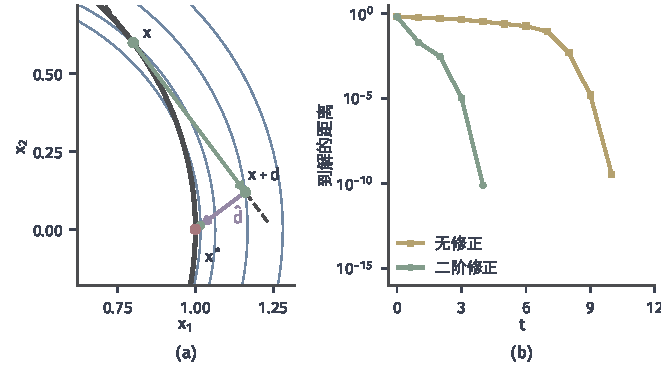
\includegraphics[width=112mm]{figures/05-optimization/06-constrained-optimization/matplotlib/sqp-maratos/figure.pdf}
 \caption{问题~\eqref{eq:sqp-maratos}上的Maratos效应与二阶修正。(a)~深灰粗线是约束，蓝线是目标的等高线，虚线是线性化约束；绿色箭头是QP步，紫色箭头是修正步$\hat{\bm{d}}$，红点是解。(b)~$\rho=2$、$\eta=0.1$的回溯SQP：不修正（黄）前七轮步长被缩短，修正（绿）后每轮都走全步。}
 \label{fig:sqp-maratos}
\end{BookInlineFigure}

\paragraph{为什么修正是二阶的}
设$\lVert\bm{d}\rVert_2$很小。约束在$\bm{x}+\bm{d}$处的值只剩二阶项，所以$\hat{\bm{d}}$的长度是$\lVert\bm{d}\rVert_2^2$的量级，比主步小一阶，不会破坏主步带来的快速收敛。

把修正后的点代入约束展开，$\bm{A}(\bm{x}+\bm{d})$与$\bm{A}(\bm{x})$之差是$\lVert\bm{d}\rVert_2$的量级，乘以$\hat{\bm{d}}$得三阶项；其余项也是三阶以上，因此修正后的违反量降到$\lVert\bm{d}\rVert_2^3$的量级。

\paragraph{与重新解QP的区别}
修正步用的是已有的$\bm{A}$和它的分解，只换了右端，代价是一次回代加一次约束求值。重新构造并求解QP则要重新求导和分解。有不等式时，修正要在主步的工作集上做，或者把线性化约束的常数项换成$\bm{g}(\bm{x}+\bm{d})-\bm{G}\bm{d}$再解一次QP，后者花费更多，但结果仍是原QP的一次扰动。

实现中通常只在全步被拒绝、且约束违反确实增加时才试一次修正，试探失败就回到回溯。也有别的办法绕开Maratos效应，例如暂时放行一步、几步之后再回头检查的非单调策略，以及改用可微的评价函数。

\section{收敛与计算成本}
\label{sec:sqp-convergence}

各个部件都有了，本节回答三个问题：在解附近能收敛多快，什么时候算结束，以及每一轮的计算花在哪里。

\paragraph{精确Hessian的局部二次收敛}
先看只含等式的情形，记$\bm{w}=(\bm{x},\bm{\nu})$。定理~\ref{thm:sqp-newton}说全步长SQP就是$\bm{F}(\bm{w})=\bm{0}$上的Newton法，其Jacobian正是KKT矩阵$\bm{K}(\bm{w})$。所以收敛性的证明与第~\ref{chap:second-order-methods}章的证明思路相同，只是矩阵不再对称正定。

\begin{theorem}[SQP的局部二次收敛]
\label{thm:sqp-local-quadratic}
设$\bm{w}^\star=(\bm{x}^\star,\bm{\nu}^\star)$满足等式约束问题的KKT条件，$\bm{A}(\bm{x}^\star)$行满秩，并且$\nabla^2_{\bm{x}\bm{x}}\mathcal{L}(\bm{w}^\star)$在$\bm{A}(\bm{x}^\star)$的零空间上正定。设在半径为$r$的球内$\bm{K}$满足
\begin{equation}
 \lVert\bm{K}(\bm{w})-\bm{K}(\bm{w}')\rVert_2\leq M\lVert\bm{w}-\bm{w}'\rVert_2.
 \label{eq:sqp-k-lipschitz}
\end{equation}
令$\sigma>0$为$\bm{K}(\bm{w}^\star)$的最小奇异值。若$\lVert\bm{w}^{(t)}-\bm{w}^\star\rVert_2<\min\{r,\sigma/(2M)\}$，则全步长SQP的下一点有定义，且
\begin{equation}
 \lVert\bm{w}^{(t+1)}-\bm{w}^\star\rVert_2\leq\frac{M}{\sigma}\lVert\bm{w}^{(t)}-\bm{w}^\star\rVert_2^2.
 \label{eq:sqp-quadratic-bound}
\end{equation}
\end{theorem}

\begin{proof}
记$\bm{e}=\bm{w}^{(t)}-\bm{w}^\star$，$\bm{K}=\bm{K}(\bm{w}^{(t)})$。定理~\ref{thm:sqp-eqp}说明$\bm{K}(\bm{w}^\star)$可逆，所以$\sigma>0$。

第一步说明$\bm{K}$的逆有界。由式~\eqref{eq:sqp-k-lipschitz}，
\[
 \lVert\bm{K}-\bm{K}(\bm{w}^\star)\rVert_2\leq M\lVert\bm{e}\rVert_2\leq\frac\sigma2.
\]
最小奇异值的扰动不超过矩阵差的范数，所以$\bm{K}$的最小奇异值至少是$\sigma/2$，即
\[
 \lVert\bm{K}^{-1}\rVert_2\leq\frac2\sigma.
\]

第二步写出误差递推。由$\bm{F}(\bm{w}^\star)=\bm{0}$沿线段积分，
\[
 \bm{F}(\bm{w}^{(t)})=\int_0^1\bm{K}(\bm{w}^\star+s\bm{e})\bm{e}\,\mathrm{d}s.
\]

下一点是$\bm{w}^{(t)}$减去$\bm{K}^{-1}\bm{F}(\bm{w}^{(t)})$，把上式代入，得到
\[
 \bm{w}^{(t+1)}-\bm{w}^\star
 =\bm{K}^{-1}\int_0^1\bigl(\bm{K}-\bm{K}(\bm{w}^\star+s\bm{e})\bigr)\bm{e}\,\mathrm{d}s.
\]

第三步估计积分。由式~\eqref{eq:sqp-k-lipschitz}，被积函数的范数不超过$M(1-s)\lVert\bm{e}\rVert_2^2$，积分后得
\[
 \Bigl\lVert\int_0^1\bigl(\bm{K}-\bm{K}(\bm{w}^\star+s\bm{e})\bigr)\bm{e}\,\mathrm{d}s\Bigr\rVert_2\leq\frac M2\lVert\bm{e}\rVert_2^2.
\]
再乘以第一步的界，式~\eqref{eq:sqp-quadratic-bound}成立。
\end{proof}

这里$M$是$\bm{K}$的Lipschitz常数，它由$f$与$h_j$的三阶导数大小和乘子的大小共同决定，当目标和约束的Hessian都Lipschitz连续时存在。由于$\lVert\bm{e}\rVert_2<\sigma/(2M)$时式~\eqref{eq:sqp-quadratic-bound}的右端小于$\lVert\bm{e}\rVert_2/2$，迭代留在球内，二次收敛一直保持。

条件各有用处。行满秩和约化曲率正定都是用来保证$\bm{K}(\bm{w}^\star)$可逆的，这正是定理~\ref{thm:sqp-eqp}的条件。注意结论是关于$\bm{w}$的。单看$\bm{x}$的误差，或单看违反量，不必单调下降，表~\ref{tab:sqp-newton-run}中$t=1$到$t=2$的$\lvert h\rvert$就几乎不动。

\paragraph{含不等式时}
由定理~\ref{thm:sqp-identification}，LICQ、严格互补和二阶充分条件下，靠近解时局部QP有一个活动集恰为$\bm{S}^\star$的解。若求解器返回这个解，SQP就和把$\bm{S}^\star$当作等式的SQP完全一样，定理~\ref{thm:sqp-local-quadratic}适用于这个等式问题，得到二次收敛。

这里有三个“若”，缺一不可：活动集已被识别，全步长被接受，并且QP求解器选中了这个解。第二点正是上一节二阶修正要保证的。

\paragraph{拟Newton的局部超线性收敛}
用近似矩阵时，分析更细。在同样的约束资格和二阶充分条件下，若迭代已收敛于解、步长为$1$，并且$\bm{B}^{(t)}$有界，式~\eqref{eq:sqp-dennis-more}是$\bm{x}^{(t)}$超线性收敛的刻画。这个结论的证明要比较拟Newton步与精确Newton步的差，篇幅较长，读者可查阅专著\scite{math-nocedal2006numerical}。

条件不会自动成立。全空间的BFGS矩阵需要沿$\bm{d}^{(t)}$的切向分量持续得到好的曲率信息，阻尼会使一部分更新偏离割线条件。已知的保证多是两步超线性这样较弱的形式，或者依赖额外的假设。图~\ref{fig:sqp-exact-bfgs-rate}中尾部的快速下降是一次运行的现象，不能当作普遍定理。

\paragraph{远离解时}
上面的结论都假定初始点已经足够接近解。远离解时依靠接受规则。对罚函数线搜索，常见的全局结论是：若迭代点留在紧集内，$f,g_i,h_j$足够光滑，约束梯度在其上一致线性无关，$\bm{B}^{(t)}$一致有界且一致正定，$\rho$最终固定下来，QP都相容，则极限点是原问题的KKT点。证明要用到式~\eqref{eq:sqp-merit-descent}给出的逐步下降以及回溯的步长下界，读者可查阅专著\scite{math-nocedal2006numerical}。过滤器有相应的结论，需要它自己的一组假设。

这种结论要求的条件不同于局部结论，得到的也只是KKT点，不是全局最优解，非凸问题上它可能收敛到鞍点甚至极大方向的驻点附近。图~\ref{fig:sqp-global-local}是问题~\eqref{eq:sqp-circle}从远处出发的运行。圆上还有另一个KKT点$(-1,-1)^\top$，那是圆上目标的最大点，乘子$\nu=-1/2$，起点$(0.2,-1.6)^\top$在圆的下方。

\begin{BookInlineFigure}
 \centering
 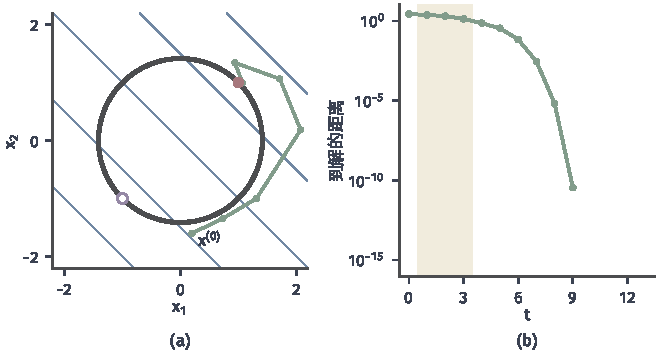
\includegraphics[width=112mm]{figures/05-optimization/06-constrained-optimization/matplotlib/sqp-global-local/figure.pdf}
 \caption{问题~\eqref{eq:sqp-circle}从$(0.2,-1.6)^\top$、$\nu^{(0)}=1$出发的回溯SQP，$\rho=1$，约化曲率不足$0.5$时移位。(a)~路径（绿）绕过圆的右侧到达解（红点），紫色空心点是圆上目标的最大点。(b)~到解的距离，黄色带是步长小于$1$的轮次，此后全步长二次收敛。}
 \label{fig:sqp-global-local}
\end{BookInlineFigure}

运行分成两个阶段。前四轮步长依次是$1,0.25,0.5,0.5$，其中第二到第五轮的约化曲率不足，加了移位，这是接受规则和曲率修正在起作用。之后步长一直是$1$，到解的距离依次为$0.347$、$0.0686$、$0.00289$、$6.7\times10^{-6}$、$3.5\times10^{-11}$，进入Newton的快速段。

\paragraph{停止准则}
“QP解完了”不是结束的标志，判断要回到原问题的KKT残差上。给定容差$\varepsilon_{\mathrm{p}},\varepsilon_{\mathrm{d}},\varepsilon_{\mathrm{c}}>0$，同时检查原始可行、Lagrange驻定和互补三项：
\begin{equation}
 \begin{gathered}
 \lVert\bm{h}(\bm{x})\rVert_\infty\leq\varepsilon_{\mathrm{p}},\qquad\lVert[\bm{g}(\bm{x})]_+\rVert_\infty\leq\varepsilon_{\mathrm{p}},\\
 \lVert\nabla f(\bm{x})+\bm{A}^\top\bm{\nu}+\bm{G}^\top\bm{\lambda}\rVert_\infty\leq\varepsilon_{\mathrm{d}},\\
 \bm{\lambda}\geq\bm{0},\qquad\max_i\lvert\lambda_ig_i(\bm{x})\rvert\leq\varepsilon_{\mathrm{c}}.
 \end{gathered}
 \label{eq:sqp-stopping}
\end{equation}
三项的单位不同，实际中要按目标与约束的尺度归一化。步长很小不能作为收敛的证据，那可能只是回溯失败。

\paragraph{一轮的成本}
表~\ref{tab:sqp-cost}按$n$个变量、$p+m$条约束的稠密情形列出一轮的主要开销。其中QP的迭代次数$k$在热启动的后期常常是$1$或很小的数，而在早期、活动集变动频繁时可能很大。

\begin{BookInlineTable}
 \centering
 \begin{tabular}{ll}
  \toprule
  项目 & 开销\\
  \midrule
  一阶导数 & $\nabla f$与$\bm{A},\bm{G}$各一次\\
  精确曲率 & $m+p+1$个Hessian或Hessian向量积\\
  拟Newton更新 & 约$O(n^2)$\\
  KKT分解（等式） & 约$O((n+p)^3)$，稀疏时远小于此\\
  工作集迭代 & $k$次，每次低秩修正约$O(n^2)$\\
  步的接受 & 每次试探$f$和约束各一次\\
  二阶修正 & 约束一次，再加一次回代\\
  恢复阶段 & 额外的模型构造与子问题求解\\
  \bottomrule
 \end{tabular}
 \caption{SQP一轮的主要开销。}
 \label{tab:sqp-cost}
\end{BookInlineTable}

和第~\ref{chap:penalty-multiplier-methods}章的方法相比，SQP每轮贵得多，一轮要解一个QP，但轮数通常很少，适合函数求值昂贵、约束数目不太大的问题。约束和变量都很多、活动集又难以确定时，分解和工作集迭代的开销变大，第~\ref{chap:nonlinear-interior-point}章的内点法每轮结构更固定，往往更合适。

\section{本章小结}
\label{sec:sqp-summary}

本章从圆周上的小问题出发，回答了章首提出的几个问题。SQP在当前点把目标近似到二阶、把约束近似到一阶，得到一个局部QP。目标的线性项来自$\nabla f$，曲率却要取Lagrange函数的Hessian，因为约束的弯曲只有通过乘子才折算得进模型。所以算法同时维护原始变量和乘子。

只含等式时，局部QP归结为一个KKT线性系统，可以整体分解，也可以分成法向段和零空间内的切向段。行满秩和约化Hessian正定保证解是模型的最小点。取精确Lagrange Hessian时，这个系统正是原问题KKT方程的Newton步。

含不等式时要决定哪些约束算数。有效集法维护工作集，步非零时用比值检验防止越界，步为零时用乘子的符号决定释放哪条约束。有效集法只是QP的一种解法，并不是SQP的一部分，QP也可以用内点法等方法求解。工作集属于当前的线性化QP，只有在约束资格、二阶充分条件和严格互补下，靠近解时才与原问题的活动集一致。

曲率方面，KKT矩阵可逆、约化Hessian正定、$\bm{B}$在全空间正定是三件不同的事。负曲率可以用移位、约化曲率修正或信赖域处理，它们分别改变模型或步长范围。拟Newton近似用同一组乘子下的Lagrange梯度差作割线，用阻尼保持正定，超线性收敛还需要沿步方向的切向曲率逐渐准确。

模型的步要放回原问题检验。罚函数把目标和违反量压成一个数，权重必须超过乘子，又不宜过大；过滤器并排比较两个指标，靠裕量、切换规则和恢复阶段才成为完整的机制。线性化约束无解时用弹性子问题或恢复阶段修复子问题，好步被弯曲约束的二阶违规挡住时用二阶修正修复候选步。恢复失败也不能证明原问题不可行。

最后要分清两类结论。解附近的快速收敛依赖约束资格、二阶充分条件、活动集的识别和全步长的接受；远离解时的可靠进展依赖接受规则和一致有界的曲率。两者条件不同，结论也不同，后者只给出KKT点，并不给出全局最优。全程都要分别检查QP的可行性与原非线性约束的可行性，前者只是后者在切平面上的影子。

